% define document type (i.e., template. Here: A4 APA manuscript with 12pt font)
\documentclass[man, 12pt, a4paper]{apa7}

% change margins (e.g., for margin comments):
%\usepackage{geometry}
% \geometry{
% a4paper,
% marginparwidth=30mm,
% right=50mm,
%}

% add packages
\usepackage[american]{babel}
\usepackage[utf8]{inputenc}
\usepackage{csquotes}
\usepackage{hyperref}
\usepackage[style=apa, sortcites=true, sorting=nyt, backend=biber, natbib=true, uniquename=false, uniquelist=false, useprefix=true]{biblatex}
\usepackage{authblk}
\usepackage{graphicx}
\usepackage{setspace,caption}
\usepackage{subcaption}
\usepackage{enumitem}
\usepackage{lipsum}
\usepackage{soul}
\usepackage{xcolor}
\usepackage{fourier}
\usepackage{stackengine}
\usepackage{scalerel}
\usepackage{fontawesome}
\usepackage[normalem]{ulem}
\usepackage{longtable}
\usepackage{amsmath}
\usepackage{afterpage}
\usepackage{float}

% Select what to do with to-do notes: 
% \usepackage[disable]{todonotes} % notes not showed
\usepackage[draft]{todonotes}   % notes showed

% make warning with red triangle
\newcommand\Warning[1][2ex]{%
  \renewcommand\stacktype{L}%
  \scaleto{\stackon[1.3pt]{\color{red}$\triangle$}{\tiny\bfseries !}}{#1}}%

% make question with red triangle
\newcommand\Question[1][2ex]{%
  \renewcommand\stacktype{L}%
  \scaleto{\stackon[1.3pt]{\color{red}$\triangle$}{\tiny\bfseries ?}}{#1}}%

% formatting links in the PDF file
\hypersetup{
pdfpagemode={UseOutlines},
bookmarksopen=true,
bookmarksopenlevel=0,
hypertexnames=false,
colorlinks   = true, %Colours links instead of ugly boxes
urlcolor     = blue, %Colour for external hyperlinks
linkcolor    = blue, %Colour of internal links
citecolor   = cyan, %Colour of citations
pdfstartview={FitV},
unicode,
breaklinks=true,
}

% language formatting
\DeclareLanguageMapping{american}{american-apa}

% add reference library file
\addbibresource{references.bib}

% Title
\title{Integration of Migrants: A Descriptive Conceptual Framework and Systematic Review}
\shorttitle{Integration of Migrants}

% Authors
\author[*,1,2]{Jannis Kreienkamp}
\author[1,2]{Kai Epstude}
\author[1,2]{Laura F. Bringmann}
\author[1,2]{Peter de Jonge}
\affiliation{\hfill}
\affil[1]{University of Groningen, Department of Psychology}
\affil[2]{Author order still to be decided (sorted alphabetically by first name)}

\authornote{
   \addORCIDlink{* Jannis Kreienkamp}{0000-0002-1831-5604}

We have no known conflict of interest to declare.

Correspondence concerning this article should be addressed to Jannis Kreienkamp, Department of Psychology, University of Groningen, Grote Kruisstraat 2/1, 9712 TS Groningen (The Netherlands).  E-mail: j.kreienkamp@rug.nl}

\leftheader{Kreienkamp}

% Abstract
\abstract{
One of the key challenges to researching acculturation is an immense heterogeneity in definitions and measures. These inconsistencies make it difficult to compare past literature on acculturation, hinder straight-forward measurement selections, and hampers the development of an overarching framework. To structure our understanding of the migration process, we propose to use the four basic elements of human experiences (motivations, emotions, thoughts, and behaviors) as a descriptive framework. We then embed this migration experience structure within the individual socio-historical context. To test our framework, we perform a systematic review and separately analyse validated scales and empirical studies in their measurements of motivational, emotional, cognitive, and behavioral acculturation aspects. We find that most scales and studies focus on behavioral and cognitive operationalisations. We inversely find that emotional and motivational aspects are measured rarely and predominantly in conjunction with other experience elements. We also find structural differences acculturation measures across publication fields. We, thus, showcase the utility of an experience-based framework in structuring our analyses and understandings of acculturation. 

[currently 166 words]
}

\keywords{Keyword \#1, Keyword \#2, ...}

% set indentation size
\setlength\parindent{1.27cm}

% Main document:
\begin{document}

% add title information (incl. title page and abstract)
\maketitle

% **CHEAT SHEET / LEGEND**
%
% Comments:
% '%' starts a comment in LaTeX (not printed)
% '\todo[inline]{} makes orange boxes in PDF
% '\marginpar{}' notes in margins
% '\footnote{}' footnote
%
% Citation (with Natbib citation style):
% '\citep[e.g.][p. 15]{CitationKey}' citation in parentheses "(e.g., Berry, 2003, p. 15)"
% '\citet{CitationKey}' citation in text "Berry (2003)"
% '\citealt' and '\citealp' alternate citation without parentheses
% '\citeauthor' and '\citeyear' only year or author
% 
% Headings:
% '\part{}' and '\chapter{}' only relevant for multi-part or multi-chapter documents
% '\section{}' heading level 1
% '\subsection{}' heading level 2
% '\subsubsection{}' heading level 3
% '\paragraph{}' heading level 4
% '\subparagraph{}' heading level 5
%
% formatting:
% '\textbf{}' text bold font
% '\textit{}' text italic font
% '\underline{}' text underline
% '\sout{}' text strike out
% '\textsc{}' text small caps
% '\vspace{1em}' add vertical space
% '\hspace{1em}' add horizontal space
% '\\' new line (i.e., line break)
% '\pagebreak' start new page (i.e., page break)
% '\noindent' do not indent current line (e.g., current paragraph)
% 'begin{center}...end{center}' center text or object
%
% Math mode:
% '$\alpha = .8$' mathematical equation inline
% '$$\hat{y} = b_0 + b_1x$$' mathematical equation in its own line
% '\begin{equation}...\end{equation}' multi-line equation
% '\approx' approximate symbol
% '\neq' not equal
% '\bar' mean bar over letter
% '\pm' plus minus sign 
% '^{}' superscript
% '_{}' subscript
% '\fraq{numerator}{denominator}' fraction
% '\sqrt[n]{}' square root
% '\sum_{k=1}^n' sum for 1 through n
%
% Insert things:
% '\input{filename}' inputs the raw (tex) file as a command (e.g., tables and R-Markdown imports)
% '\include{filename}' includes section on new page (incl. possible auxiliary info)
% '\includegraphics[settings]{filename}' add a figure or graph
% '\caption{}' adds a caption to a table or figure
% '\label{}' labels sections, tables, figures, etc. so that they can be referred to.
% '\ref{}' refer to a labelled sections, tables, figures, etc.
% '\begin{enumerate}...\end{enumerate}' numbered list
% '\begin{itemize}...\end{itemize}' bullet-ed list
% '\item' item in list section 
%
% Symbols:
% '\&' and sign
% '\%' percent sign
% '\_' three dotes
% '\#' hash symbol

%% Relevance:
Migration is a complex human experience of change and the process of adapting to this change. The adaptation of migrants in new cultural contexts is an important issue in many societies around the world. With many of the migration push and pull factors in the economic, safety, social, and environmental domains worsening, the topic is likely to become even more important in the future (\hl{Reference}).
The current challenges and increasing migration highlight once more how important it is to understand how adaptation processes unfold and which aspects are most important to positive and sustainable outcomes. 

%% Problem:
% Heterogeneity leads to challenges of: comparison, inclusion/focus decision in research and interventions, and overarching framework
One of the fundamental challenges to psychological integration, faced by researchers, practitioners, and policy-makers, is an essentially scattered field with immense heterogeneity in definitions and measures of individual cultural adaptation
\footnote{\textbf{I know this is way too long and we should probably just use `acculturation' and make a note that we mean the original meaning.} Researchers have used a wide range of terms in the context of cultural interactions, including acculturation, enculturation, transculturation, assimilation, integration, and cultural adaptation, -adjustment, or -transition. While there are often important conceptual differences between the terms, they all aim to capture and describe a process of change when two cultures interact. In this paper we will mostly use the term \textit{cultural adaptation}. The term `adaptation' in its etymology takes a functional approach -- where both individuals and interactive systems adjust to be better suited for their environment. In this understanding, cultural adaptation is (1) relevant on an individual- and a group level, (2) places responsibility on any individual and group in the environment, and (3) is inherently a temporal and interactive process. Note that we do not specify what exactly is adaptive in any circumstance and that 'adaptation' is not a necessary outcome (i.e., many change processes do not enhance the livability of groups or individuals). Cultural adaptation rather seems to be a target that underlies most measures and definitions in the field. We also want to highlight that the term (psychological) acculturation was originally referred to as a neutral and descriptive umbrella term, which shares many of these attributes (e.g., \citealp{Berry2003}). Yet, we chose not to use acculturation as our primary term because over the past 90 years users of the term have most frequently used it in a static manner \citep{Brown2011, Ward2019} and have placed disproportional responsibility on migrants \citep{Bourhis1997a} -- despite its more neutral original intention \citep[e.g.,][]{Berry2009a}. We believe that part of this confusion stems from the word itself, where the ac- prefix indicates a movement (of an individual) towards a cultured end-state. Yet, because the term \textit{acculturation} is often used in the psychological literature and the term \textit{integration} is widely used in societal debates, we will, at times, use these terms interchangeably with cultural adaptation.}.
The inconsistency of included and excluded aspects brings researchers and practitioners to face fundamental challenges when (1) looking back at past literature and interventions, because it becomes hard to compare different effects and outcomes, (2) when looking forward, it becomes hard to choose a definition and measurement for new research and intervention efforts, and (3) more generally, the scattered state of the literature hampers the development of an overarching framework.

%% Solution/Aim:
% Propose and test a framework to analyse, measure, and understand cultural adaptation.
The aim of this paper is, therefore, to offer a descriptive conceptual framework to analyse, measure, and understand the concept of individual cultural adaptation. Such a framework has a different objective than previous efforts to catalogue literature on cultural adaptation \citep[e.g.,][]{Castels2003}, build multidimensional measures of integration \citep[e.g.,][]{Harder2018}, normative frameworks \citep[e.g.,][]{Ager2008a}, or theories of acculturation \citep[e.g.,][]{Berry2005}. Rather than offering a new measurement, definition, or theory, we aim to build a framework to assess and compare any of these conceptual elements. 
We propose to do so by using the basic elements of human experiences and motivation to structure the concept of cultural adaptation.
Once we have introduced our conceptual framework, we will systematically review the past methodological and applied empirical literature on acculturation to apply our framework and tests its utility. \\

\section{The Framework: Embedded Migration Experiences}
%% Structure of the section: 
% Both widely applicable structuring but also context.
The utility of a conceptual framework arguably depends on its ability to comprehensively structure a concept and to do so across a wide range of contexts. Yet, at the same time, the contexts should not remain a black box. In the following sections we will, thus, introduce both our structuring framework and our conceptualization of context in more detail (also see Figure \ref{fig:ModelContext} for an overview).

\begin{figure}[h]
\centering
\caption{Conceptual Model with Context. Too complex, static, and not enough focus on our key elements?}
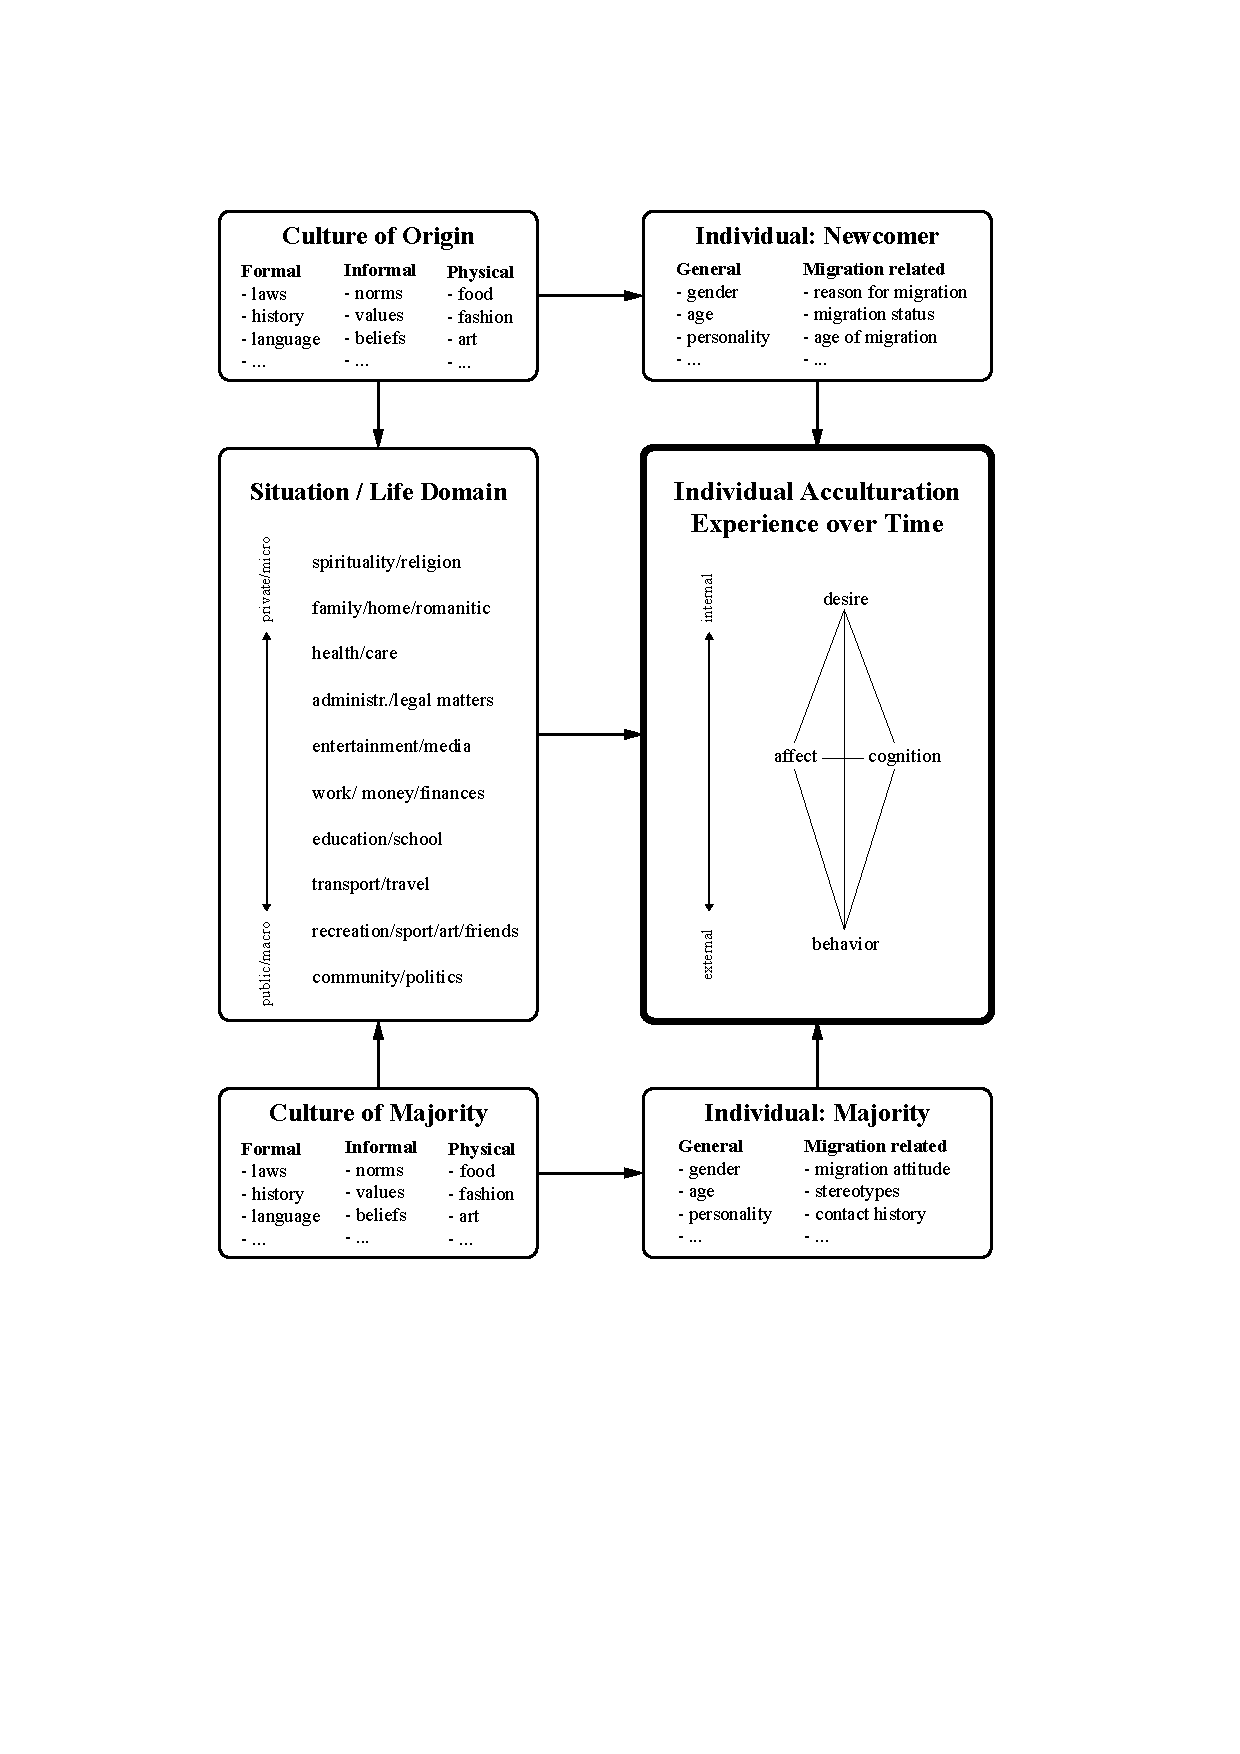
\includegraphics[width=\textwidth]{Figures/ConceptualFrameworkStatic.pdf}
\label{fig:ModelContext}
\end{figure}

\subsection{The Migration Experience}
%% Proposal: 
% Use human experience to structure our understanding of cultural adaptation.
To build a framework that captures the complex process of cultural adaptation and is applicable across a heterogeneous field, we chose to focus on basic psychological faculties relevant to all human beings --- across contexts and time scales. A growing body of literature suggests that any human experience can be understood as a set of needs, emotions, cognitions, and behaviors \citep[sometimes referred to as the ABCs or ABCDs of psychology: affect, behavior, cognition, desire; e.g.,][]{Cottam2010, Hogg2005, Jhangiani2014}. Following the premise that any human experience can be perceived within these four basic elements, we propose that the migration experience (i.e., cultural adaptation) can also be structured as a set of motives, emotions, thoughts, and behaviors. 

%% Example: 
% Examples of ABCD in cultural adaptation.
Cultural adaptation in this framework might, for example, be understood or measured in terms of behavioral adaptation, such as language use, or voting; cognitive adaptation, such as identification with cultural values; affective adaptation, such as feeling at home, or loneliness; motivational adaptation, such as the satisfaction of competence or independence needs; or as a complex combination of any or all of these aspects. 

%% Features of Experience Framework: 
% ABCD comprehensively captures experience, is a scale-able evaluation, and universally relevant across contexts.
Using the building blocks of human experiences not only ensures that the framework comprehensively captures the entire migration experience, but experiences are also relevant across time-scales, because experience perceptions are scale-able evaluations --- of a single situation, a recent period, or a life-long journey (\hl{Reference}).
Moreover, there is also evidence that ABC(D) frameworks are universally relevant for all human beings\footnote{For a detailed discussion of the distinction between \textit{universalism} and \textit{absolutism} see \citet{Berry2000, Berry2009a}.}. The frameworks have, for example, been found across cultures \citep[e.g.,][]{Bhawuk2011} and likely structure human forebrain functioning \citep{Swanson2020}\footnote{It should also be noted that ABC(D) frameworks have been used effectively to structure theories and models across a wide variety of fields --- including research on attitudes \citep{Breckler1984} and ambivalence \citep{VanHarreveld2015}, self-regulation \citep{Ben-Eliyahu2015}, the big five personality traits \citep{Wilt2016}, suicidality \citep{Harris2015} and in clinical interventions \citep{Eifert1989}, and even the review of acculturation literature \citep{Ward2001, Ward2019}. Interestingly, the affect, behavior, and cognition structure has even found application in the development of human-like machines \citep{Guo2020}.}.

%% Application: 
% Universality of elements allows us to ask: Which aspects have been considered? How many aspects have been considered? And which have been considered together?
% In this study we ask answer these questions for past literature.
These attributes of comprehensiveness, scale-ability, and universality are ideal for comparing and assessing different definitions and measurements in past and present literature. It allows us to ask questions such as: Which aspect of the migration experience has been considered as part of acculturation in a particular research project? Which aspect is measured most frequently in a certain field? Or what is the average number of aspects included in definitions or measurements? 
In the current paper, we will test some of these questions for the past empirical literature. In particular, we will assess which aspects of cultural adaptation have most frequently been included. And which aspects are most frequently considered together. We will also assess how many of the motivational, emotional, cognitive, and behavioral aspects are measured within the studies. Moreover, to assess differences between fields, we will also group past research based on the journals' target audience. 
% interesting: call for unpublished data or check in theses, whether different ABCD composition.

%% Experience as Critical Research Tool: 
% Thinking about experience forces you to take the perspective of your research participants.
Before we move on to the context of the migration experience, we would like to remark on a few important nuances of the framework. One important emphasis of the experience conceptualization is that it is inherently a bottom-up approach to the topic. Taking migration experiences as the starting-point highlights the considerations for the lived realities of the researched individuals and communities. Scholars in the traditions of critical research methods have long highlighted the importance of including the participants in the research conceptualization process \citep[e.g.,][]{Kovach2009}. If one uses the experiences of the researched individuals to guide the study questions and design, one inevitably emphasizes the agency and needs of the community -- lending relevance and ownership of knowledge to the community \citep[e.g., ][]{Schmidt2021}.

%% Experience Content:
% we focus on structure not on content.
One further important distinction is that while anyone will have motives, emotions, thoughts, and behaviors, what one needs (e.g., belongingness or independence), feels (e.g., sadness or happiness), thinks (e.g., identification or disinterest), or does (e.g., studying or working) is highly ideographic. It is this ideographic content that makes the framework relevant to such a broad range of migration contexts. Yet it is the content-free structure (i.e., the presence or absence of the basic elements) that is transferable across contexts and studies, enabling comparisons and broader conceptual discussion. In this paper, we will thus focus on the the latter structuring properties of the experience framework. That is, we will, for example, assess whether migrant behaviors or emotions were considered but not which behaviors or emotions were considered in particular. This allows us to start a broader discussion of the type cultural adaptation experience considered across the scattered field (inversely, considerations of particular emotions and behaviors will likely be important to considerations of individual studies of contexts).

\subsection{The Context}
%% Introduction context: 
% Experience depends on what is permitted by culture, situation, individual background, and time in the migration process.
The perceptions of an experience are often fundamentally influenced by the context and environment. Which perceptions a situation permits (i.e., contextual affordances) has long been a topic of discussion in the field of ecological psychology \citep[e.g.,][]{Cantor1994}. Recent efforts to formalize the structure of contexts have, for example, highlighted the interactive process of group-environments and individuals \citep[e.g.,][]{Young2002}.
Adjacent to the discussions in ecological psychology, we would like to address four contextual factors in particular: (1) Cultures, (2) individuals, (3) situations, and (4) the process.

\subsubsection{Culture} 
% culture: patterns of social arrangements in society
% Note to self - Émile Durkheim: 
% institutions (family, government, economy, media, education, healthcare, and religion) and 
% social facts (formal: law, regulations, policies, history, language; informal: norms, values, beliefs, [e.g., roles, moral-, religious beliefs], rituals, customs, cultural products: fashion, architecture, arts [e.g., film, music, literature, art])

%% Introduction Culture: 
% Culture is prominent and should be structured for a widely applicable framework.
The most prominent contextual factor of cultural adaptation is probably the role of the interacting cultures. The role of culture seems particularly important, because it becomes salient in our social lives and influences a wide variety of attitudes and behaviors, but also in social structures and institutions. 
Most (semi-)applied research projects might not need to consider or formalize the structural role of cultures -- because they can simply embed their research in the cultural context of the two particular cultures they considered.
But theories of acculturation and broader social- and cultural theories have long considered different conceptual influences of culture and society on the individual's experience. We will rely on these theories to guide our understanding of culture here. However, because our framework fundamentally relies on the individual acculturation experience, we will merely use the structuring elements of these sociological, anthropological, and psychological theories. Moreover, because these fields often use different terms to describe the same or similar concepts, our presentation here might not always be consistent with the original terminologies. Similarly, the individual theoretical and philosophical positions and implications (and their criticisms) would be beyond the scope of our paper and will thus not be discussed here.

% Culture as social facts: social facts (formal: law, regulations, policies, history, language; informal: norms, values, beliefs, [e.g., roles, moral-, religious beliefs], rituals, customs, cultural products: fashion, architecture, arts [e.g., film, music, literature, art]) relate to the affordances of ABCD
In our attempt to structure the influences of \textit{culture} we will mainly use extensions on Émile Durkheim's concept of \textit{social facts} \citep[e.g.,][]{Durkheim1982, Gilbert1989} and Berry's \textit{general framework of acculturation} \citep{Berry1997b, Berry2003, Berry2006a}. Interestingly, Durkheim's original definition of the concept of social facts directly referred to affect, behavior, and cognition (and potentially desires), when he wrote that social facts ``consist of manners of acting, thinking and feeling external to the individual, which are invested with a coercive power by virtue of which they exercise control over him'' (p. 52). Following this definition, we will mainly consider external (cultural or societal) influences that guide a person's motivational, cognitive, emotional, and behavioral experience. Within the sociological literature, these social influences can be divided into the formal social facts (e.g., laws, regulations, policies, history, language), informal social facts \citep[e.g., norms, values, beliefs, rituals, customs; also see][]{Herzog2018}, as well as more material cultural products or artifacts \citep[e.g., food, fashion, architecture, or arts, such as film, music, literature, and fine arts; e.g., see][]{Alexander2001}. The content of these external influences will likely be relevant in the expected patterns of behavior (e.g., dress or communication styles), cognition (e.g., sense of race-, class-, gender-, and sexual identities), emotions (e.g., expressions of emotions), and motivations (e.g., virtues and duties).

% Interaction of multiple cultures: Use Berry to highlight power imbalances of where once culture might be more influential than another.
In the case of cultural adaptation (at least) two sets of cultural arrangements will be influencing the experience of the individual. Quite a substantial body of literature has considered this interaction between the two cultures. For our conceptualization we will use Berry's framework for acculturation research \citep[e.g., see][p. 15, Fig. 2]{Berry1997b} and Berry's acculturation framework for stress and adaptation \citep[e.g., see][p. 45, Fig. 4.1]{Berry2006a}, because they explicitly propose to jointly consider the cultural influences on the ``acculturation experience'', which we consider here (see Figure \ref{fig:ModelContext}). Once we consider this encounter of multiple cultures within the structure of culture as social facts, it also becomes apparent that there are usually considerable power imbalances between the cultures \citep[e.g., see][]{Bhatia2001}. This imbalance is especially apparent in formal or material elements, such as laws or language, but similarly extends to more informal elements, such as default expectations in communication or behavioral norms and customs. Factors such as cultural distance \citep{Triandis2001} or majority group's attitudes \citep[e.g.,][]{Berry1997b, Berry2003} might, of course, influence such power imbalances, but the structuring of both acculturation and culture encourages and facilitates reflections and discussions of these issues. As part of the analyses presented in this paper, we will offer such a reflection by extracting the cultures for which acculturation measures were validated and investigated in empirical papers. This allows us to examine how much the external influences of culture on motives, emotions, thoughts, and behaviors are reflected within structural differences of measures and definitions (that is, if we can consolidate a meaningful number of studies per cultural context).

\subsubsection{Individual} 
% Individual based on intergroup contact and Berry: Individual differences in general (e.g., age, gender) but also migration related differences (e.g., reason for migration, language proficiency)
Another contextual factor to consider during the cultural adaptation process are the interacting individuals themselves. There has been a rising focus on the idea that acculturation centers around the daily interpersonal interactions a person has with people of the other group \citep{Maxwell2017, Sam2010}. And although it can, at times, be difficult to disentangle cultural from individual influences, there are a range of personal features that likely influence the cultural adaptation process. These personal differences might relate to relatively stable individual differences, such as gender or personality, but also migration related differences, such as the reason for migration (e.g., voluntary vs. forced migration), cultural distance, or migration status. Within the migration related factor we would also include aspects that might change over the course of the adaptation process but give migrants different starting positions, such as language skills and education level.
Similar to the influences of cultures, the individual differences of the interaction partners (if there are multiple people) will likely impact the cultural adaptation. And similar to culture, individual differences likely play a role for multiple aspects of the cultural adaptation process (also see Figure \ref{fig:ModelContext}). As part of this study, we will mainly analyze the migration relevant differences. Considering individual differences on a larger, cross-study level we will mainly extract data on the type of samples collected within the validation and the empirical papers (e.g., forced vs. voluntary, youth, or clinical samples). If we find reasonable numbers of studies with specific types of samples, we will assess whether these individual differences are related to structural differences in measures or definitions used by the authors.

\subsubsection{Situation} 
% Situations as domains of psycho-social functioning: Many theories have come up with life domains that form different cultural interaction situations.
Beyond the cultural group and the individuals, the interactions of cultural adaptation are further dependent on the situational context. One way of structuring this situational context is what we will here refer to as the \textit{domains of psycho-social functioning} -- the idea that the social experience will take place within different domains in life. There are many social-scientific theories that have discussed these spheres of life. One famous example is Bronfenbrenner's Ecological systems theory \citep{Bronfenbrenner1992}, according to which humans get into contact with others, and society at large, through a number of environmental systems that range from the closest relations (e.g., family or colleagues) to the more remote relationships (e.g., mass media or societal services). A similar framework was suggested by prominent theorists of the (structural) functionalist traditions with the concept of social institutions \citep[e.g.,][]{Turner1997}. According to these sociological theorists, it is through societal institutions (commonly: family, government, economy, media, education, healthcare, and religion) that culture is transmitted and maintained \citep[e.g.,][]{Durkheim1982}. Similar ideas for domains of interaction with society and culture have also been proposed within the acculturation literature. \citet{Arends-Toth2006, Arends-Toth2007} have, for example, suggested 15 public and private life domains (e.g., education [public], child-rearing [private]) in which acculturation takes place. Empirical research in the individual acculturation field, have also provided evidence that acculturation processes can develop separately and differently within these domains \citep[e.g.,][]{Arends-Toth2003a}. 

% point of convergence: We aggregate a list of micro to macro domains from past literature.
What structurally unites the conceptualizations of life domains is the dimension of closeness to the individual. That is, most areas of life found in the literature can be arranged from the most immediate (i.e., micro or private, such as family) to the broadest levels (i.e., macro or public, including government or media). So, based on sociological theories of social institutions \citep{Durkheim1982}, literature on life domains in acculturation \citep{Arends-Toth2006, Arends-Toth2007, Zane2004}, a categorization of psychological influences by the British Psychological Society \citep{Michie2005a}, and Bronfenbrenner's Ecological systems theory \citep{Bronfenbrenner1992}, we conceptualized a range of life domains relevant to the migration process (see Figure \ref{fig:ModelContext}). Interestingly, most methodological and empirical authors mention explicitly which domains of acculturation they measure or very clearly focus on a limited number of domains in their measurement or definition of acculturation. As part of this study we will, therefore, extract information on the domains mentioned and measured in the literature. We will then assess whether different foci on life domains also show differences in their understanding and measurement of the motivational, emotional, cognitive, and behavioral cultural adaptation.

\subsubsection{Process} 
% Dynamic process rather than static end-product: Experience can answer this call because it can only be understood based on past experiences
A final, fundamental factor we would like to address in the cultural adaptation framework is the understanding of cultural adaptation as a dynamic process rather than a static end-product. That cultural adaptation is a developmental process, and that ``acculturation occurs when two independent cultural groups come into \textit{continuous first-hand contact over an extended period of time}'' \citep[][186]{Berry1989} seem to be a generally accepted assumption within the field. Yet, within the empirical literature, few studies have actually considered the theoretical implications of migration as a process and even fewer have methodologically followed the trajectories of migrants over time. Recent years have seen a growing awareness of this discrepancy \citep[e.g.,][]{Brown2011, Ward2019}. We believe that the experience framework of cultural adaptation, as it is presented here, is ideally suited to deal with this conceptualization as a developmental process. Philosophers of the phenomenological tradition have long highlighted that subjective experience can only be understood within the history of past experiences \citep[e.g.,][; also see Figure \ref{fig:ModelContext}]{Heidegger1867}. In this study we apply our interest in the role of time by extracting the types of analyses (static vs. dynamic) done by the authors, and assessing whether data was collected prior to migration, after migration, or both. We will then also assess whether different traditions of data collection show differences in their understanding and measurement of the motivations, emotions, thoughts, and behaviors aspects of cultural adaptation (if the systematic review includes a reasonable number of longitudinal studies).

\section{The present study}
The aim of our empirical efforts presented here is to put our proposed framework to the test. We have lamented that one of the challenges of a heterogeneous field is that it is difficult to assess and compare past literature. As a framework, we have suggested that the psychological elements of experiences could comprehensively structure our assessment of the literature. We will thus retrieve the past psychological literature that has proposed or used a measure of cultural adaptation and we will extract which experiential elements were considered in the research. We expect that these efforts will provide insights into the perceived importance of motives, emotions, cognitions, and behaviors for cultural adaptation. We also expect that this allows us to assess how many experience aspects are usually considered and which aspects are considered jointly. And finally, we aim to compare the understanding of cultural adaptation across different contexts and fields. 

To test the utility of the framework, we specifically target the measurement of cultural adaptation as an operationalization of the concept within the empirical literature. We will first consider methodological literature, which aims to develop acculturation measures. Validated scales usually focus on a concept in detail rather than cherry-picking aspects relevant to an `applied' study. Yet, coding cultural adaptation measures separately might also aid future considerations of measure selection because we would effectively build a data base of scales that can be filtered by whether the scale includes measurements of motives, emotions, thoughts, or behaviors. Once we have considered the validated scales in particular, we will further assess the empirical literature that measures of cultural adaptation in general. Thus, in the following section we will briefly discuss how we extract key information from the literature and will then sequentially analyze the role of experience elements in the methodological and broader empirical literature of psychological cultural adaptation.

\Question\ Potentially Paragraph on: Why not meta analysis? (main problem: comparability across studies. Too diverse and scattered but also at different places in the model)

\section{Systematic Review}
\todo[inline]{Search Strategy}
To assess the past psychological literature on cultural adaptation, we performed a systematic review. On March 4\textsuperscript{th}, 2020, we searched for empirical work on the acculturation of migrants within the ``APA PsycInfo'' bibliographic databases via the EBSCO\textit{host} provider (for the full information on the search strategy see Appendix \ref{app:AppendixSearchStrategy}). We downloaded all references and abstracts which two independent coders screened for relevance -- first based on the titles and then based on the abstracts. We downloaded all relevant and available works for full-text coding. We used this database to identify validated scales in the literature as well as empirical work in general. For both groups of work we extracted a range of variables to test our framework. Before we describe each of the two data sets in more detail we will briefly lay out how we extracted the variables for our main analyses. The full coding process and data extraction is described in the online supplementary materials X (as well as on OSF [citation to public osf and/or github repository goes here]).

\subsection{Framework Coding}
For our main tests of the proposed framework we extracted data on the experience elements as well as the experience context.
\subsubsection{Experience Elements}
One major focus of our coding efforts was identifying the experience elements that were assessed within each manuscript. For each article we, thus, retrieved the items used and coded whether the measure included references to emotions (affect), behaviours, cognitions, and needs. Because this concerned the most central aspect of our framework, each manuscript was double-coded and inconsistent codes were resolved after discussion. Examples of how individual aspects were identified and coded are in Table \ref{tab:DimensionExamples}.
\begin{table}[hbt]
\caption{Examples for Dimensions of Acculturation Coding}
\label{tab:DimensionExamples} 
\begin{tabular}{lll}
\hline
Dimension & Concept & Wording \\ 
\hline
Affect & belonging, loneliness, satisfaction  & "I feel ...", \\
Behavior  & \begin{tabular}[c]{@{}l@{}}language learning, media consumption,\\ 
voting\end{tabular} & "I do ...", "I speak ...", "I meet ..." \\ 
Cognition & \begin{tabular}[c]{@{}l@{}}cultural identification, cultural values,\\ 
attitude towards majority\end{tabular} & \begin{tabular}[c]{@{}l@{}}"I prefer ...", "I think ...", \\
"I identify as ..."\end{tabular} \\ 
Desire    & needs, goals, wants & \begin{tabular}[c]{@{}l@{}}"I want ...", "I would like to ...", \\
"I need ..."\end{tabular} \\ 
\hline
\end{tabular}
\end{table}


At this stage we also noted if measures included concepts that are complex and relate to multiple experience aspects. We also noted if the measures would not consider an individual’s experiences, such as simply reporting of migration status or length of residency. \Question\ What else should be noted?

\subsubsection{Experience Context}
As part efforts to capture the migration context we were interested in cultural, individual, situational, as well as process related contexts. Assessing these contexts in a manner that is relevant across a wide range of studies is challenging and likely superficial at best. Context is arguably more relevant if one considers a single case, yet gaining a more general understanding of the contexts frequently considered in the literature could prove useful in evaluating and comparing conceptions of cultural adaptation. We, thus, extracted a range of general context variables from the empirical literature.

\paragraph{Country}
To capture the cultural contexts, we coded both the heritage country of the migrants as well as the country of the receiving host society. Coding the two societal contexts allows us to extract information on the specificity of the studies (e.g., Mexican migrants in the United States, or any migrant in Scandinavia). Migrant and host country codings could also reveal patterns of `interest within the literature' (e.g., common migrant groups, common host societies, or common combinations investigated). And finally, if common clusters emerge, we could compare the types of experience elements assessed within each cluster (e.g., focus on behavioral adaptation in one and cognitive focus in another cluster). 

\paragraph{Sample}
To capture the individual background on a cross-paper level, we extract the types of samples recruited by the authors. Some studies might focus on young or elderly samples, men or women only, clinical samples, or authors might simply recruit any migrant from a certain country or region. Clusters and differences in the experience foci within these clusters might offer insights into the understanding of cultural adaptation for different individual contexts.

\paragraph{Life Domains}
To capture the situational focus of the authors, we coded which life domains the scales referred to. There were a range of ways in which we could identify the domains the authors wished to cover. Often times authors will explicitly mention which life domains there measure aims to capture. Others will show their domain focus as part of labelled sub-scale labels or factor labels. If there is no explicit mention by the authors, question are likely worded to clearly refer to a specific life domain (e.g., behaviors at school, or values in the family context). If there is no clear reference to a life domain or the questions are about life in general, we code this as meaningful information as well. We can then process the situational foci as a list of domains, which offers information on the diversity of domains (e.g., number, or similarity of domains) but also the focus in the literature in general (e.g., frequency of domain across all articles). If clusters of similar focus domains emerge, we could, additionally, assess differences in the assessment of cultural adaptation for these clusters.

\paragraph{Migration Time}
To capture the process focus, we also coded which migration step(s) the authors focused on. We coded whether the authors focused on the migration experience after the arrival in the new society, prior to the migration, or focused on both time points. We, additionally, coded whether cross-sectional or longitudinal data was collected and how this data was analyzed. Given the observations of past reviews \citep[e.g.,][]{Brown2011, Ward2019}, we expect that most researchers will collect cross-sectional data at a single time-point after migration.

\subsection{Methodological Literature}

Based on the systematic review and its coding, the first data set we
assess is a database of scale validations. We bring together the scales
suggested in previous reviews as well as validation studies we
identified in our own review. Throughout our literature review we found
five major works that reviewed the measurement of acculturation
\citep{Celenk2011, Maestas2000, Matsudaira2006, Wallace2010, Zane2004}.
After removal of duplicate scales, we added any scale validation that
was present in our own systematic review but not included in the
previous reviews. For each measure we extracted the full item list as
well as the item scoring prior to coding. A comprehensive and
interactive database of the scales, with reference- and publication
information, as well as our experience elements and -context coding is
available in our online supplementary information as well as on our open
science repository (\hl{OSF and/or github citation here}).

\subsubsection{Methods}

Taken together these five reviews collected a total of 197 scales, of
which 75 were duplicates. From our own review we added 25 additional
validation studies. After removing duplicates this meant that we
considered a total of 122 unique scales for our coding. Of these scales
we ultimately had to exclude 41, because they were either not accessible
or did not fit the the topic of our review (see Table
\ref{tab:ScalesExclusion}). The scales had an average of \hl{X.XX} items
and \hl{X.XX} sub-scales. Most items were rated on a five-point
(\hl{XX.XX}\%) or four-point likert-type scale (\hl{XX.XX}\%), with only
\hl{X} scales including categorical ratings. About a fifth of scales
(20.49\%) included majority group members in their validation studies.
The earliest included validation was from 1972 with a majority of scales
being validated around the turn of the 21\textsuperscript{st} century
and the latest included validation study in 2018.

\begin{table}

\caption{(\#tab:ScalesExclusion)Reasons for Exclusion}
\begin{tabular}[t]{lc}
\toprule
Exclusion Reason & Frequency\\
\midrule
not migration & 14\\
items not included & 8\\
search pending & 5\\
not accessible & 4\\
not found & 3\\
not acculturation & 2\\
majority focussed & 1\\
not found probably the same as Tsai et al. 2000 & 1\\
only language (no scale) & 1\\
same as S-029 & 1\\
uses other scale & 1\\
\bottomrule
\end{tabular}
\end{table}


\subsubsection{Results}

For the scale validations, we assessed both the role of experience
elements in the measures as well as contextual differences.

\paragraph{Experience}

With our main aim of examining the experience structure within the
scales, we examined whether scales included a specific experience
elements but also examined the used elements in their complex
combinations. In terms of general inclusion of elements, most studies
included a measure of cognition (89.66\%) and behavior (82.76\%),
whereas only roughly half the studies included a measure of affect
(55.17\%) and only a fourth of the scales included a measure of motives
(28.74\%). However, only a minority of scales included only a single
dimension. There were only 5 scales that exclusively relied on
cognitions (5.75\%) and 4 scales that measured only behaviors (4.6\%).
Yet, inversely, there were also only 13 scales that measured all four
dimensions (14.94\%). Most studies measured two (37.93\%) or three
(36.78\%) dimensions. A majority of scales either measured behavioral
and cognitive elements (26.44\%) or behavioral, cognitive, and affective
elements (26.44\%; also see Figure \ref{fig:ElementsScales} and Table
\ref{tab:ScaleElementCooccurrences}). Looking at the number of elements
measured together we also see substantial differences in what kind of
scales include a certain element. Scales that included cognitions
measured an average of 2.67 elements, scales measuring behavior, on
average, measured a 2.71, while scales that included affect measures had
a complexity average of 3.1 and scales measuring motivation even
measured an average of 3.4 scales. Thus, most scales measure multiple
dimensions, yet they focus on easily accessible dimensions (i.e.,
behavior and cognition), less of what is considered `less accessible' or
`subjective' (i.e., affect and desires). This is also visible in the
circumstance that there were no scales that exclusively measured
motivational or emotional adaptation (while this was the case for both
cognitions and behaviors). And if emotional or motivational aspects were
measured they were on average measured in scales that were already more
complex (i.e., included more experience elements).

\begin{figure}[h]
\centering
\caption{Scales: Bar graph of the experience element combinations.}
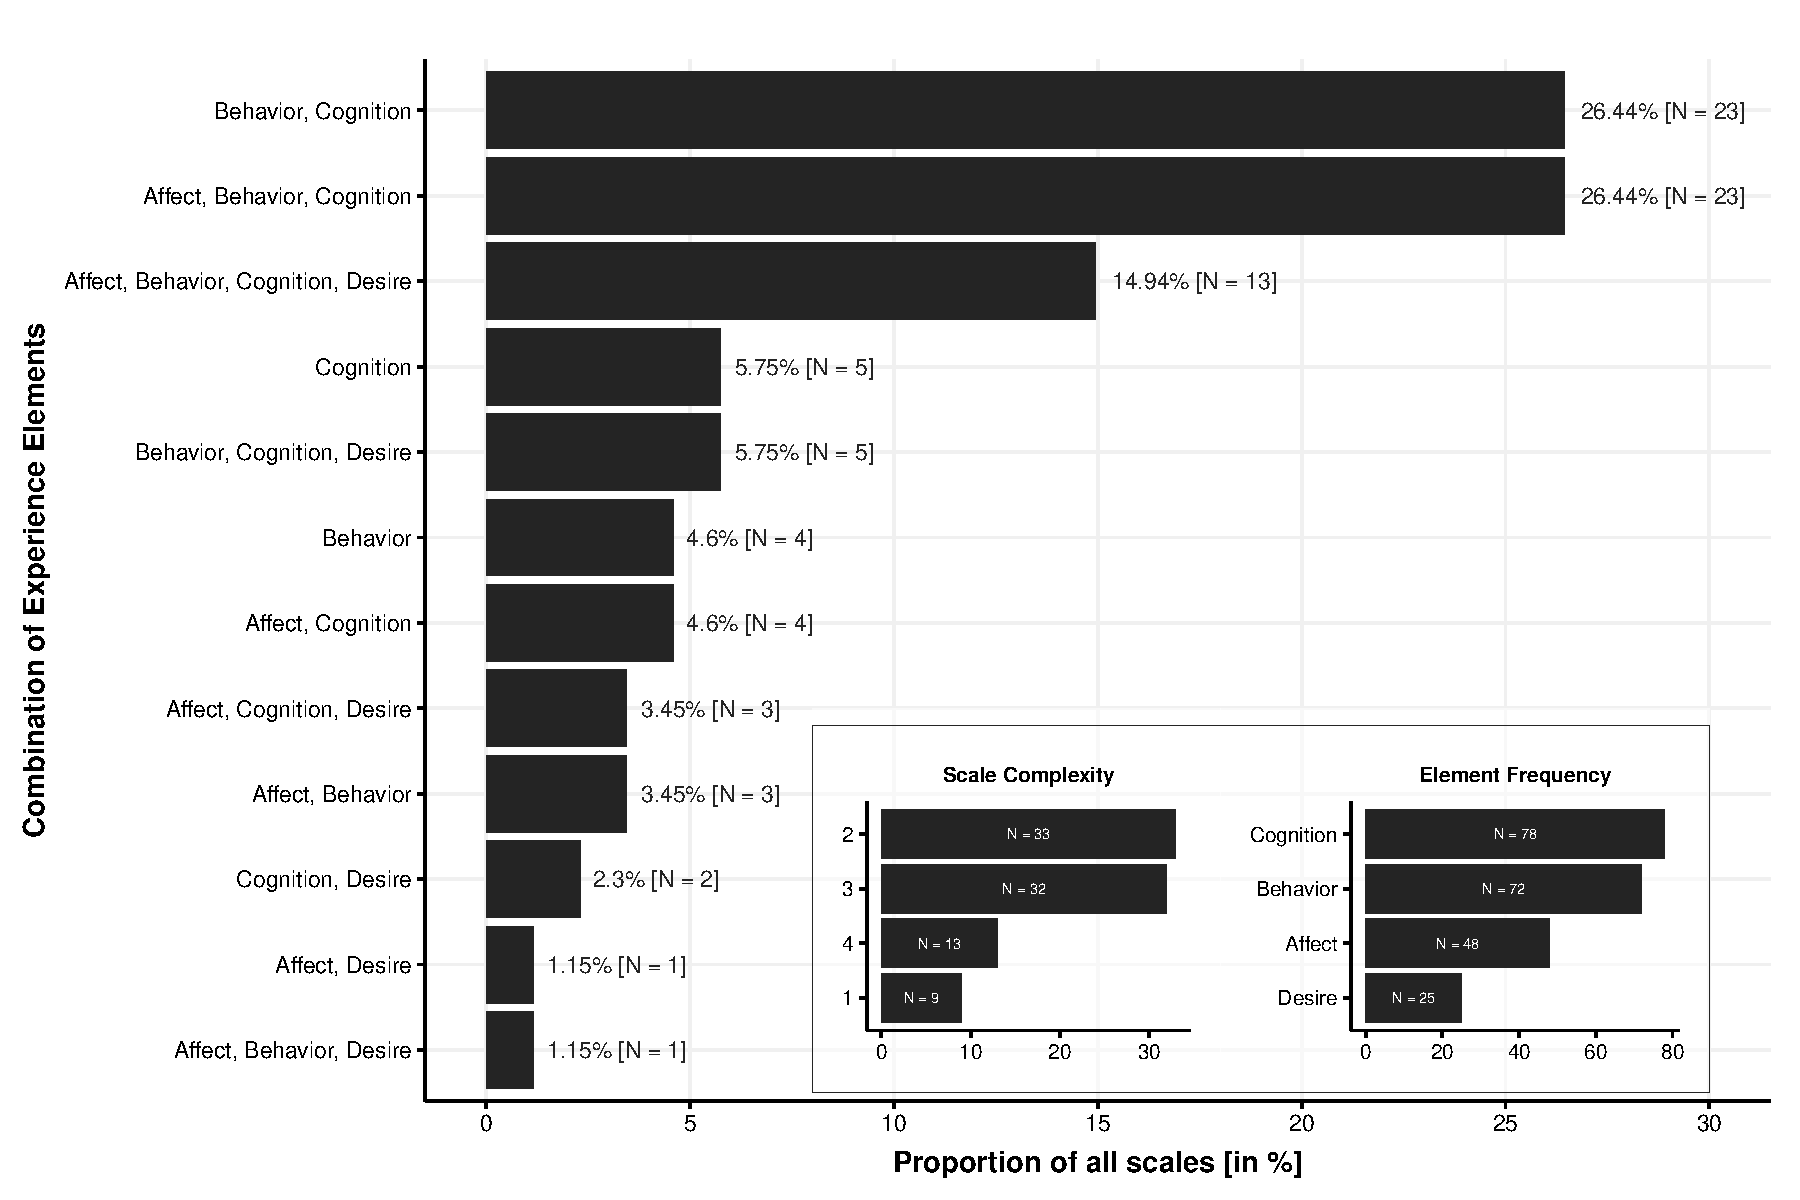
\includegraphics[width=\textwidth]{Figures/ABCDFreq-1}
\label{fig:ElementsScales}
\end{figure}

\begin{table}

\caption{\label{tab:ScaleElementCooccurrences}Scales: Element Co-occurrence Matrix}
\begin{tabular}[t]{lcccc}
\toprule
  & Affect & Behavior & Cognition & Desire\\
\midrule
Affect & 48 & 40 & 43 & 18\\
Behavior & 40 & 72 & 64 & 19\\
Cognition & 43 & 64 & 78 & 23\\
Desire & 18 & 19 & 23 & 25\\
\bottomrule
\end{tabular}
\end{table}

\paragraph{Context}

To gain a general understanding of contextual factors within the
validated studies, we also assessed cross-study patterns of cultural,
individual, situational, and process-related focus points.

\subparagraph{Country}

To assess the cultural contexts for which scales were validated, we
assessed the migrants' countries of settlement as well as the countries
of origin. We found that most scales investigated a single host country
(\textit{N} = 81) and most investigated one country of origin
(\textit{N} = 68). There were only 3 scales that were validated for more
than one receiving country. Additionally, there was one study with two
scales that were validated with the origin culture as the starting point
(i.e., single origin country, multiple host countries). Looking at the
country patterns, we found that an overwhelming number of scales were
validated within a U.S. American settlement context (\textit{N} = 61).
But also the remaining receiving societies were mostly `western'
countries (e.g., Canada, The Netherlands, The United Kingdom, Israel,
Australia) with non-western settlement contexts, such as Taiwan, Nepal,
or Russia, not being investigated across more than one study. For the
migrant origin societies there was slightly more variation. There were a
few migrant groups that were investigated specifically (e.g., Mexico:
14, China:7, South Korea: 4), however most validation studies targeted
broader categories of migrants (any migrants: 11, Asian: 5, Hispanic: 9,
LatinX: 5). This also made it difficult to identify patterns of cultural
combinations investigated (apart from Mexican and LatinX migrants in the
United States).

\subparagraph{Sample}

To assess the role different groups of individuals targeted in the scale
validations, we coded the types of samples recruited for the validation
studies. A majority of studies sampled any consenting adult from the
migrant group of interest (\textit{N} = 50). As seems common in academic
research, a larger portion of the validated scales relied on young
migrants or students (\textit{N} = 29). Interestingly, only small
minority of validated scales targeted more vulnerable groups, such as
clinical samples (\textit{N} = 2) or refugees (\textit{N} = 2) --
despite a considerable focus on these groups within the broader
literature.

\subparagraph{Domains}

To assess the situational focus within the validated scales, we assessed
the number of domains within each scale as well as more common domains
across the scales. A relatively large number of scales asked about the
current state of the migrant in general manner without mentioning any
context or life domain (\textit{N} = 24; e.g., `'In general, in what
language do you read and speak?'`). The remaining scales referred to an
average of 3.49 dimensions (\textit{SD} = 3.42, range: 1 -- 21). A total
of 179 unique domains was measured across the 87 scales. The domains of
'language` (\hl{XX}\%), 'food' (\hl{XX}\%), `interactions' (\hl{XX}\%),
`family' (\hl{XX}\%) and `values' (\hl{XX}\%) were focused on most often
(see Online Supplementary Materials \hl{X}, Figure \hl{X}). Thus, while
there was large variation between the scales in the number, and
diversity of domains, the most frequently mentioned domains were in line
with the life domains proposed in the literature
\citep[e.g.,][]{Arends-Toth2007}.

\vspace{1em}
\todo[inline]{Should be re-coded to test our proposed domains. Also, re-check `general' code}

\subparagraph{Migration time}

All scales were validated using cross-sectional data after the migrant
arrived in the settlement society. This is in line with observations by
previous reviews of the field \citep[e.g.,][]{Brown2011}.

\subsection{Empirical Literature}

After analysis of the scales validations, we assessed the broader
empirical works we collected within the systematic review. We first
looked at all available empirical publications (incl.~books, chapters,
and dissertations). We later also assessed differences between fields
the work was published in. However, because we considered the fields on
an audience level, we used only empirical journal articles -- for which
journal-level audience data is available.

\subsubsection{Methods}

The search produced a total of \hl{XXX} results to which we added
\hl{XX} articles through contacts with experts in the field. We
subsequently screened out results that did not fit into our review.
After duplicate removal (\(N_{excluded}\) = \hl{XX}, \(N_{screened}\) =
484), we excluded 92 results in the title screening as well as an
additional 126 results during the abstract screening. Of the remaining
266 results, 259 papers presented empirical work on acculturation and
were coded. The 7 non-empirical results were reviews, which were not
coded because they did not fit into our coding schema. During the full
text coding we excluded an additional 26 results because they were
either not relevant or were not accessible (for exclusion reasons see
Table \ref{tab:EmpiricalExclusion} and for our PRISMA diagram see Figure
\ref{fig:PRISMA}).

\begin{figure}[h]
\centering
\caption{PRISMA diagram. Position still undecided. Currently generated in R based on n(row) maybe make prettier. \Warning\ Re-check numbers before duplicates removed and number of papers added from other sources.}
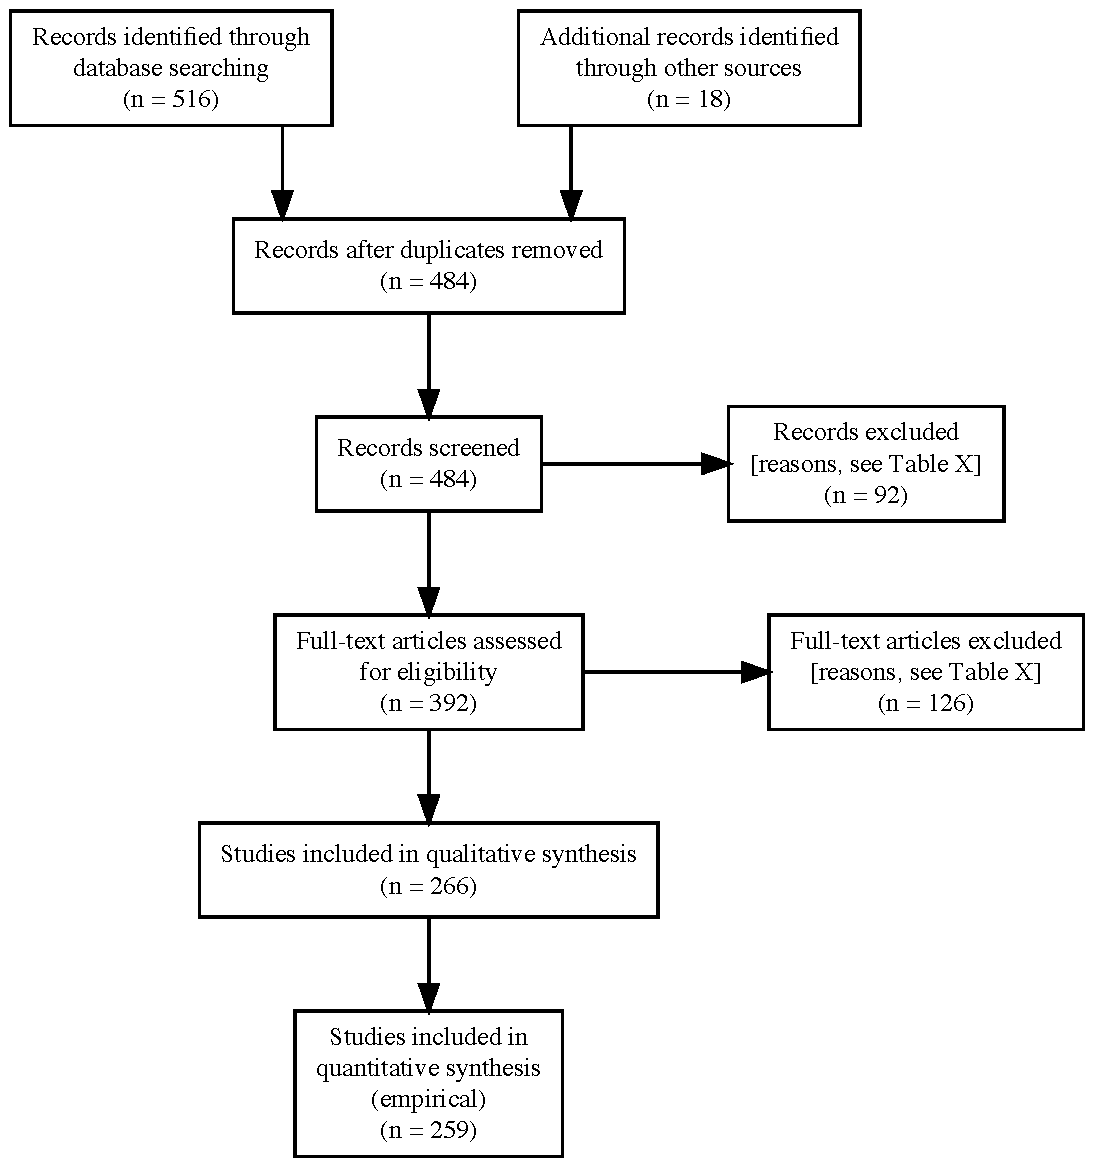
\includegraphics[width=\textwidth]{Figures/PRISMA}
\label{fig:PRISMA}
\end{figure}

\begin{table}

\caption{\label{tab:EmpiricalExclusion}Exclusion Reasons Empirical Literature}
\centering
\begin{tabular}[t]{lccc}
\toprule
\multicolumn{1}{c}{ } & \multicolumn{3}{c}{Screening} \\
\cmidrule(l{3pt}r{3pt}){2-4}
Exclusion Reason & Title & Abstract & Full Text\\
\midrule
not migration & 36 & 27 & \\
not acculturation & 19 & 49 & \\
not experience & 19 & 24 & \\
not migrant & 17 & 18 & \\
not measured &  & 8 & 2\\
re-migration &  & 1 & \\
thesis not accessible &  &  & 13\\
book not accessible &  &  & 4\\
items not accessible &  &  & 4\\
article not accessible &  &  & 2\\
should still be coded &  &  & 1\\
\bottomrule
\end{tabular}
\end{table}


Of the final works we coded, 192 were journal articles, 37 theses, and 4
book chapters. Most studies presented quantitative data (\textit{N} =
205), mixed methods (\textit{N} = 14), or qualitative data (\textit{N} =
11), while the remaining 3 manuscripts were reviews of empirical data. A
vast majority of the authors used the term `acculturation' (or
derivative versions, such as `acculturation attitudes' or `acculturation
orientation'; \textit{total N} = 178), or `integration' (\textit{N} = 7)
to refer to cultural adaptation. Notably, a majority of the empirical
investigations did not share common measures of cultural adaptation --
186 studies used measures that were reported a maximum of five times,
with a considerable majority of papers using new or ad-hoc measures of
cultural adaptation. Only about every tenth study included the local
majority in the study (\textit{N} = 25, 10.8225\%). Cultural adaptation
most frequently was a predictor variable (\textit{N} = 99, 42.8571\%), a
dependent variable (\textit{N} = 72, 31.1688\%), or a correlation
variable (\textit{N} = 27, 11.6883\%) in the empirical works. This
pattern was mirrored when looking at the focus of the papers, where a
majority of the papers had acculturation as their main focus (\textit{N}
= 83, 36.7257\%), with other bodies of work focusing on health outcomes
(\textit{N} = 23, 10.177\%), or inter-group relations (\textit{N} = 12,
\texttt{empFocusRelationPerc}\%) as their main outcomes. The earliest
included study was published in 1970, with a continuous increase of
publications after the year 2000, with considerable publication peaks in
2011 and 2019. We provide full descriptions of descriptive data
extractions and additional information about the data description in
Online Supplementary Information X.

\paragraph{Field of Publication}

For the broader empirical literature, we also collected additional data
on the field the studies were published in. To assess the differences
between fields we merged the `Scimago Journal Ranking Database'
\citep{SCImago2020} with our empirical review. For all available journal
articles we added information on key journal metrics (incl.~H index,
impact factor, and data on the field and audiences). This also meant
that dissertations, book chapters, and books were excluded from this
analysis because data on their publishers is not readily available or
unreliable. Additionally, 8 journals were not included in the Scimago
database (likely because they do not have an ISSN identifier or were
discontinued before 1996, see Online Appendix \hl{X}, Table \hl{X} for
the missing journals). We ultimately had journal metrics for 183
empirical articles. The Scimago database classifies each journal
according to the field(s) that the journal aims to address. Importantly,
(1) each journal can be be classified to address multiple fields and (2)
the field include codes of fields (e.g., `Social Sciences') as well as
sub-fields (e.g., `Social Psychology'). This leads to the case that
there can be substantial overlap between fields, and journals cannot
easily or readily be assessed in mutually exclusive subgroups.

To summarize the articles further we then classified the field
combinations into super-ordinate discipline codes. These discipline
codes are based in part on U.S. Department of Education's subject
classifications \citep[i.e., CIP;][]{InstituteofEducationSciences2020},
the U.K. academic coding system
\citep[JACS 3.0;][]{HigherEducationStatisticsAgency2013}, the Australian
and New Zealand Standard Research Classification
\citep[ANZSRC 2020;][]{AustralianBureauofStatistics2020}, as well as the
Fields of Knowledge project \citep{ThingsmadeThinkable2014}. We
ultimately classified each journal into one of four mutually exclusive
disciplines (psychology: \textit{N} = 61, multidisciplinary: \textit{N}
= 57, Medicine, Nursing, and Health: \textit{N} = 51, and Social
Sciences (miscellaneous): \textit{N} = 14. For a full discussion of the
classifications see Online Supplementary Materials \hl{X}).

\subsubsection{Results}

To test the utility of our framework, we again assessed the role of
experience elements in the measurement as well as contextual
differences.

\paragraph{Experience}

In terms of the overall frequencies of experience elements, the broader
empirical data mirrored that of the validation studies. Most studies
included a measure of cognition (83.26\%) and behavior (80.69\%),
whereas only about half of all studies included a measure of affect
(51.93\%) and only a fifth of the studies included a measure of motives
(18.45\%). Yet, only 42 studies focused on a single element
(\(N_{behavior\ only}\) = 20, \(N_{cognition\ only}\) = 18,
\(N_{emotion\ only}\) = 4). Similarly, only 17 papers included measures
of all four experience elements (7.3\%). Most studies measured three
(37.77\%) or two dimensions (36.91\%). Different from the scale
validations, within the broader empirical works most works included
measures of emotions, behaviors, and cognitions (\textit{N} = 69,
29.61\%), with a further substantial number of articles measuring
behaviors and cognitions (\textit{N} = 53, 22.75\%. Also see Figure
\ref{fig:EmpPlotFreq-1} and Table
\ref{tab:EmpiricalElementCooccurrences}). Looking at the number of
elements measured together we again see substantial differences in what
kind of scales include the individual elements. Scales that included
cognitions measured an average of 2.53 elements, scales measuring
behavior, on average, measured a 2.52, while scales that included affect
measures had a complexity average of 2.86 and scales measuring
motivation even measured an average of 3.23 scales. Thus, interestingly,
not a single study measured only motivation, and measures of motives
remained mostly limited to scales that were already multidimensional.
The results exacerbate the pattern found in the scale validations,
complex measures and conceptions of acculturation are seen infrequently
and readily accessible (i.e., less subjective) dimensions of cognition
and behavior remain the focus of most studies.

\begin{figure}[h]
\centering
\caption{Empirical Literature: Bar graph of the experience element combinations.}
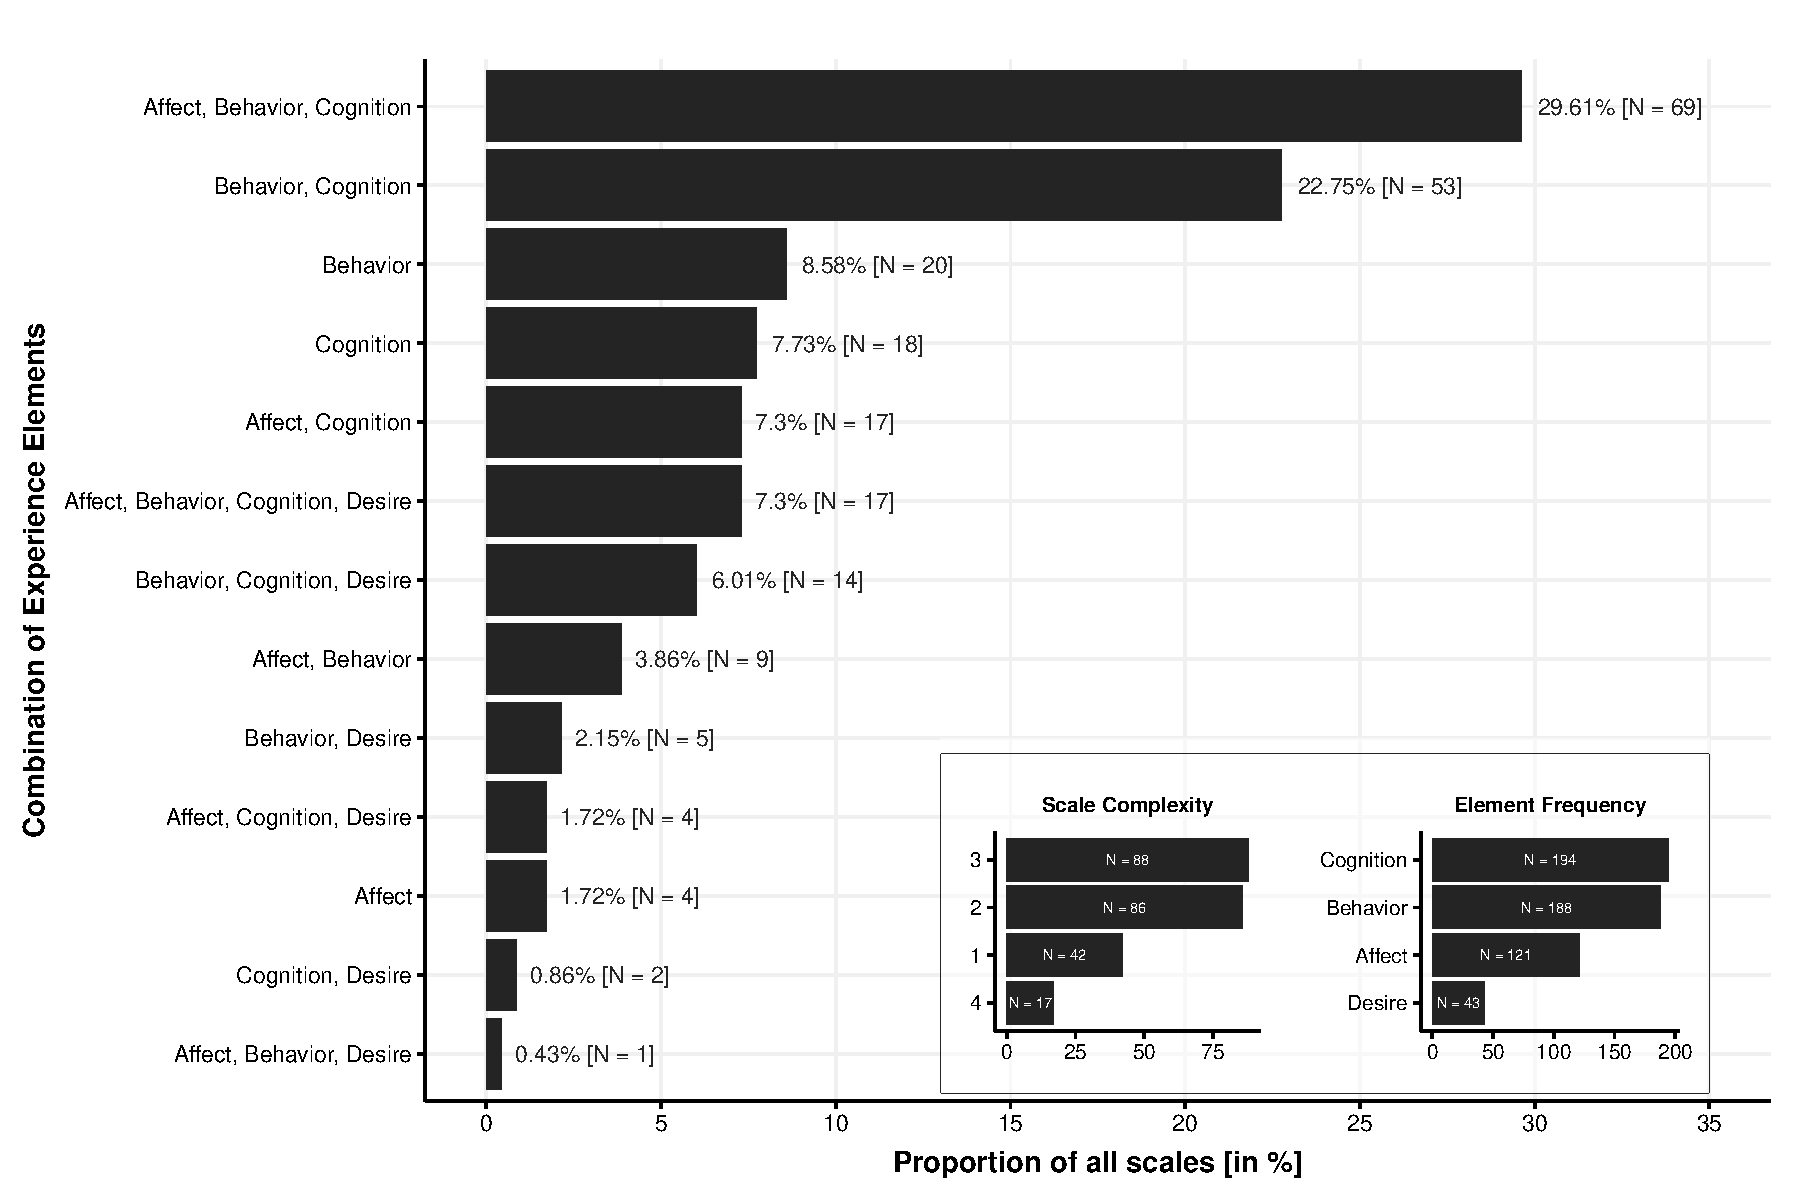
\includegraphics[width=\textwidth]{Figures/EmpPlotFreq-1}
\label{fig:EmpPlotFreq-1}
\end{figure}

\begin{table}

\caption{\label{tab:EmpiricalElementCooccurrences}Empirical Literature: Element Co-occurrence Matrix}
\centering
\begin{tabular}[t]{lcccc}
\toprule
  & Affect & Behavior & Cognition & Desire\\
\midrule
Affect & 121 & 96 & 107 & 22\\
Behavior & 96 & 188 & 153 & 37\\
Cognition & 107 & 153 & 194 & 37\\
Desire & 22 & 37 & 37 & 43\\
\bottomrule
\end{tabular}
\end{table}


\paragraph{Context}

To gain a general understanding of contextual factors within the broader
empirical studies, we again assessed cross-study patterns of cultural,
individual, situational, and process-related focus points.

\subparagraph{Country}

To assess the cultural contexts on which the authors focused, we again
assessed the migrants' countries of settlement as well as the countries
of origin. Similar to the validations, an overwhelming number of scales
were validated within a North American settlement context (United
States: \textit{N} = 109, Canada: \textit{N} = 26). But also the
remaining receiving societies were mostly `western' -- Western Europe
(e.g., The Netherlands, United Kingdom, Germany, Italy, Spain),
Australasia (Australia, New Zealand), Russia, and Israel. And only 10
studies focused on data from multiple receiving societies.

When it came to the migrants' country of origin, a majority of studies
were indifferent to migrants background and simply recruited any
consenting migrant (\textit{N} = 37), or recruited a category of
migrants (e.g., LatinX or Hispanic: \textit{N} = 21, African: \textit{N}
= 10). Among the individual countries target there was a particular
focus on the east and south-east Asian region (e.g., China: \textit{N} =
21, South Korea: \textit{N} = 19, Vietnam: \textit{N} = 11). Yet,
different from the scale validations, there was a large variety of
different origin countries that were included in less than five studies
(\textit{N} = 101 regions were targeted less than five times). Thus, the
receiving countries mainly mirrored those for which scales were
validated, yet there was an extensive number origin countries which were
investigated individually or migrants were considered irrespective of
their cultural origin. Moreover, it was again not possible to identify
distinct cultural adaptation clusters within the literature (that would
be large enough to compare).

\subparagraph{Sample}

To assess the role different groups of individuals targeted in the
empirical work, we again coded the types of samples recruited for the
studies. A majority of studies sampled any consenting adult from the
migrant group of interest (\textit{N} = 145, 62.23\%). Of the targeted
sampling strategies, most recruited refugees (\textit{N} = 22, 9.44\%),
young migrants (\textit{N} = 20, 9.01\%), or elderly people (\textit{N}
= 14, 6.01\%). The remaining fifth of the studies recruited other more
specific samples (e.g., nurses, athletes, Muslims). Interestingly,
despite the circumstance that a large portion of papers focused on
mental health outcomes, only 7 studies (3\%) recruited clinical migrant
samples. These results speak to the case that relatively few empirical
studies actually take individual differences into account in their
sample selection. Studies may still address individual differences
within the data description and within the modeling approaches (e.g.,
controlling for gender), yet it seems that inter-sectional
idiosyncrasies did not seem to play a major role in the targeting of
samples.

\subparagraph{Domains}

To capture the situational focus of the authors, we coded which life
domains the utilized measures referred to. A relatively large number of
studies assess cultural adaption in general manner without mentioning
any context or life domain (\textit{N} = 116). The remaining studies
referred to an average of 2.16 dimensions (\textit{SD} = 2.69, range: 1
-- 21)). We found a total of 183 unique domains across the 233 studies.
The dimensions of `language` (\hl{XX}\%), 'food' (\hl{XX}\%), `social
interactions,' and `friends' (\hl{XX}\%) were included most frequently.
So, while larger proportion of studies ask about cultural adaption in
general (outside of a specific domain), the number of domains included
and addressed is extensive and diverse. The mentioned domains at times
go beyond the life fields mentioned in previous work (also see Online
Supplementary Materials \hl{X}).

\vspace{1em}
\todo[inline]{Should be re-coded to test our proposed domains. Also, re-check `general' code}

\subparagraph{Process}

To assess the process focus of the broader empirical works, we again
assessed when in the migration process was collected and we additionally
assessed the type analysis done by the authors. We found that a 224
studies (96.97\%) collected cross-sectional data after the arrival of
the migrant in the new society. A single study targeted potential
migrants and 6 studies collected data prior and following the migration
event. Moreover, only 3 studies included longitudinal data analyses
concerned with cultural adaptation. This observation, again underscores
the arguments made by authors, who have long pointed out that the
acculturation literature has thus far failed to provide data that
meaningfully captures migration as a process
\citep[e.g.,][]{Brown2011, Ward2019}.

\paragraph{Fields}

To further test the utility of our framework in comparing
conceptualizations, we assessed differences of experience elements
across different fields. We provide more elaborate descriptions of the
differences in the methods, and publication types as well as contextual
differences in terms of sampling procedures, situational domains,
process-focus, analyses, and cultural contexts in Supplementary Online
Material \hl{X}.

We again first, assessed the references to affect, behavior, cognition,
and desires separately, within each of the disciplines. We find that for
all fields motivations (14.29-22.95\% of all measures in the field) and
emotions (42.86-55.74\%) are the least frequently measured elements and
each of the fields measures similarly often (in proportional terms).
However, for the cognitive and behavioral elements the proportions
diverge between the fields. While the multidisciplinary field measured
behaviors (78.95\%) and cognition (80.7\%) almost equally often, in the
medical and general social science journals behaviors were measured
considerably more often than cognitions (\(Behavior_{SoSci}\) = 100\%
\textgreater{} \(Cognition_{SoSci}\) = 50\%; \(Behavior_{Med}\) = 90.2\%
\textgreater{} \(Cognition_{Med}\) = 76.47\%). While the psychological
journals cognitions (91.8\%) were measured more often than behaviors
(70.49\%; also see Figure \ref{fig:FieldPlotFreq} B and A)).

When looking at differences in how many different elements were measured
(i.e., element complexity) and patterns within these
element-combinations, differences between the fields become increasingly
evident (also see Figure \ref{fig:FieldPlotFreq} A and C). While
`affect, behavior, and cognition' and `behavior, and cognition' measures
are the most common combinations across all fields (also at similar
proportional importance), there is less dimension complexity and
variation for medical and social science fields. In the psychological
85.25\% of all studies measures at least two experience elements
(\textit{M} = 2.41, \textit{SD} = 0.68). Although mean complexity
differences were not significantly different between the fields
(\textit{F}(3, 179) = 0.63, \textit{p} = 0.599), looking at the
qualitative differences of element combinations can be informative. For
example, there was not a single study published in a psychological
journal that conceptualized cultural adaptation by behavior alone
(eventhough this is the third most common measures in the other three
fields, also see Figure \ref{fig:FieldPlotFreq} A). Similarly, in the
broader social scientific journal desires are always measured together
with behaviors, which is very uncommon in the other
fields\footnote{Although it should be noted that the social science field was smaller and more heterogeneous than the other fields. \Warning\ Maybe drop this argument -- based on only two studies.}.
There are also interesting pattern when one considers how many other
elements an aspect is measured with within each of the fields. For
example, while for all fields motivations are found in the most complex
scales
\footnote{except for the broader social science journals that do not have many motivational measures to begin with.},
medical journal have a substantially higher average scale complexity
when measuring motivations. Inversely, psychological journal on average
report behavioral measures of cultural adaptation in more complex
scales. This hints to a pattern, where complexity might indicate
relative importance of an aspect within the field -- where only scales
that already have a broad and diverse measure also include the elements
that are usually measured less within a field (also see Figure
\ref{fig:FieldElementComp}). There are like other and more nuanced
differences in the conceptualizations highlighted within this analysis
(e.g., patterns relevant to a single field). Yet, the immediately
visible pattern differences clearly speak the utility of the framework.

\begin{figure}[h]
\centering
\caption{Combinations of measured experience element and their frequencies per field.}
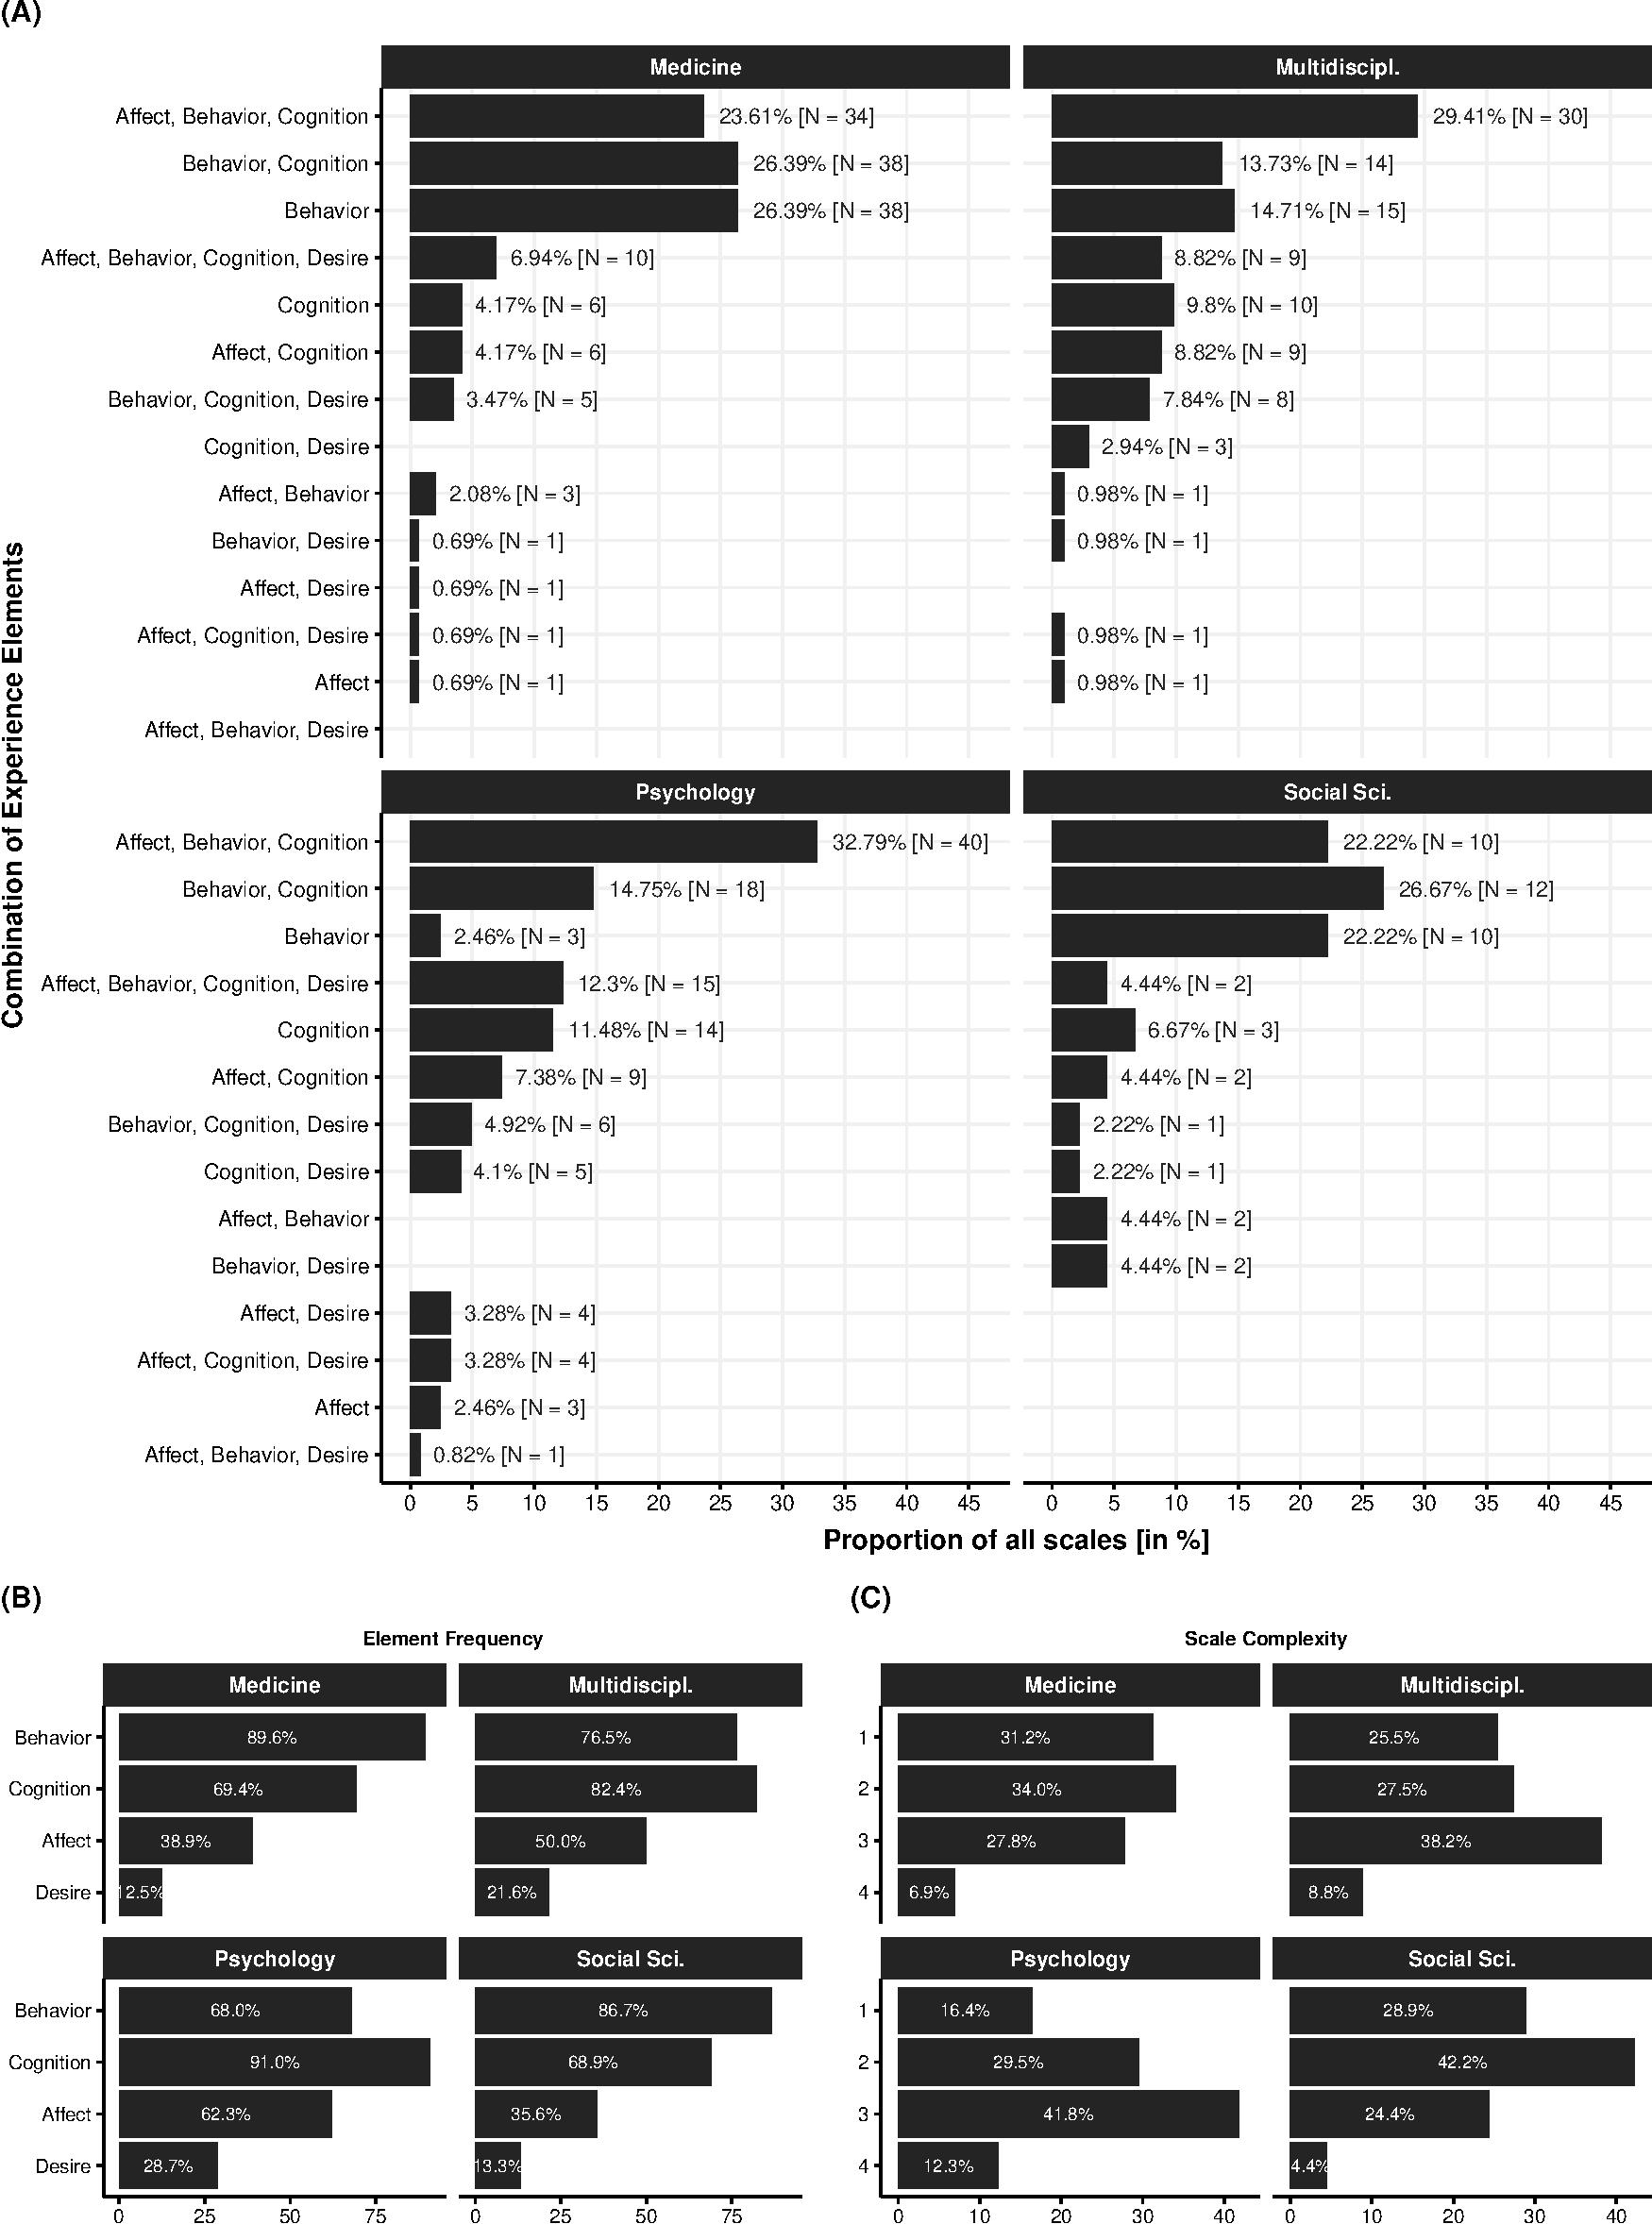
\includegraphics[width=\textwidth]{Figures/FieldPlotFreq-1}
\label{fig:FieldPlotFreq}
\end{figure}

\begin{figure}[h]
\centering
\caption{Average complexity (number of experience elements measured) for all scales that include a given experience aspect.}
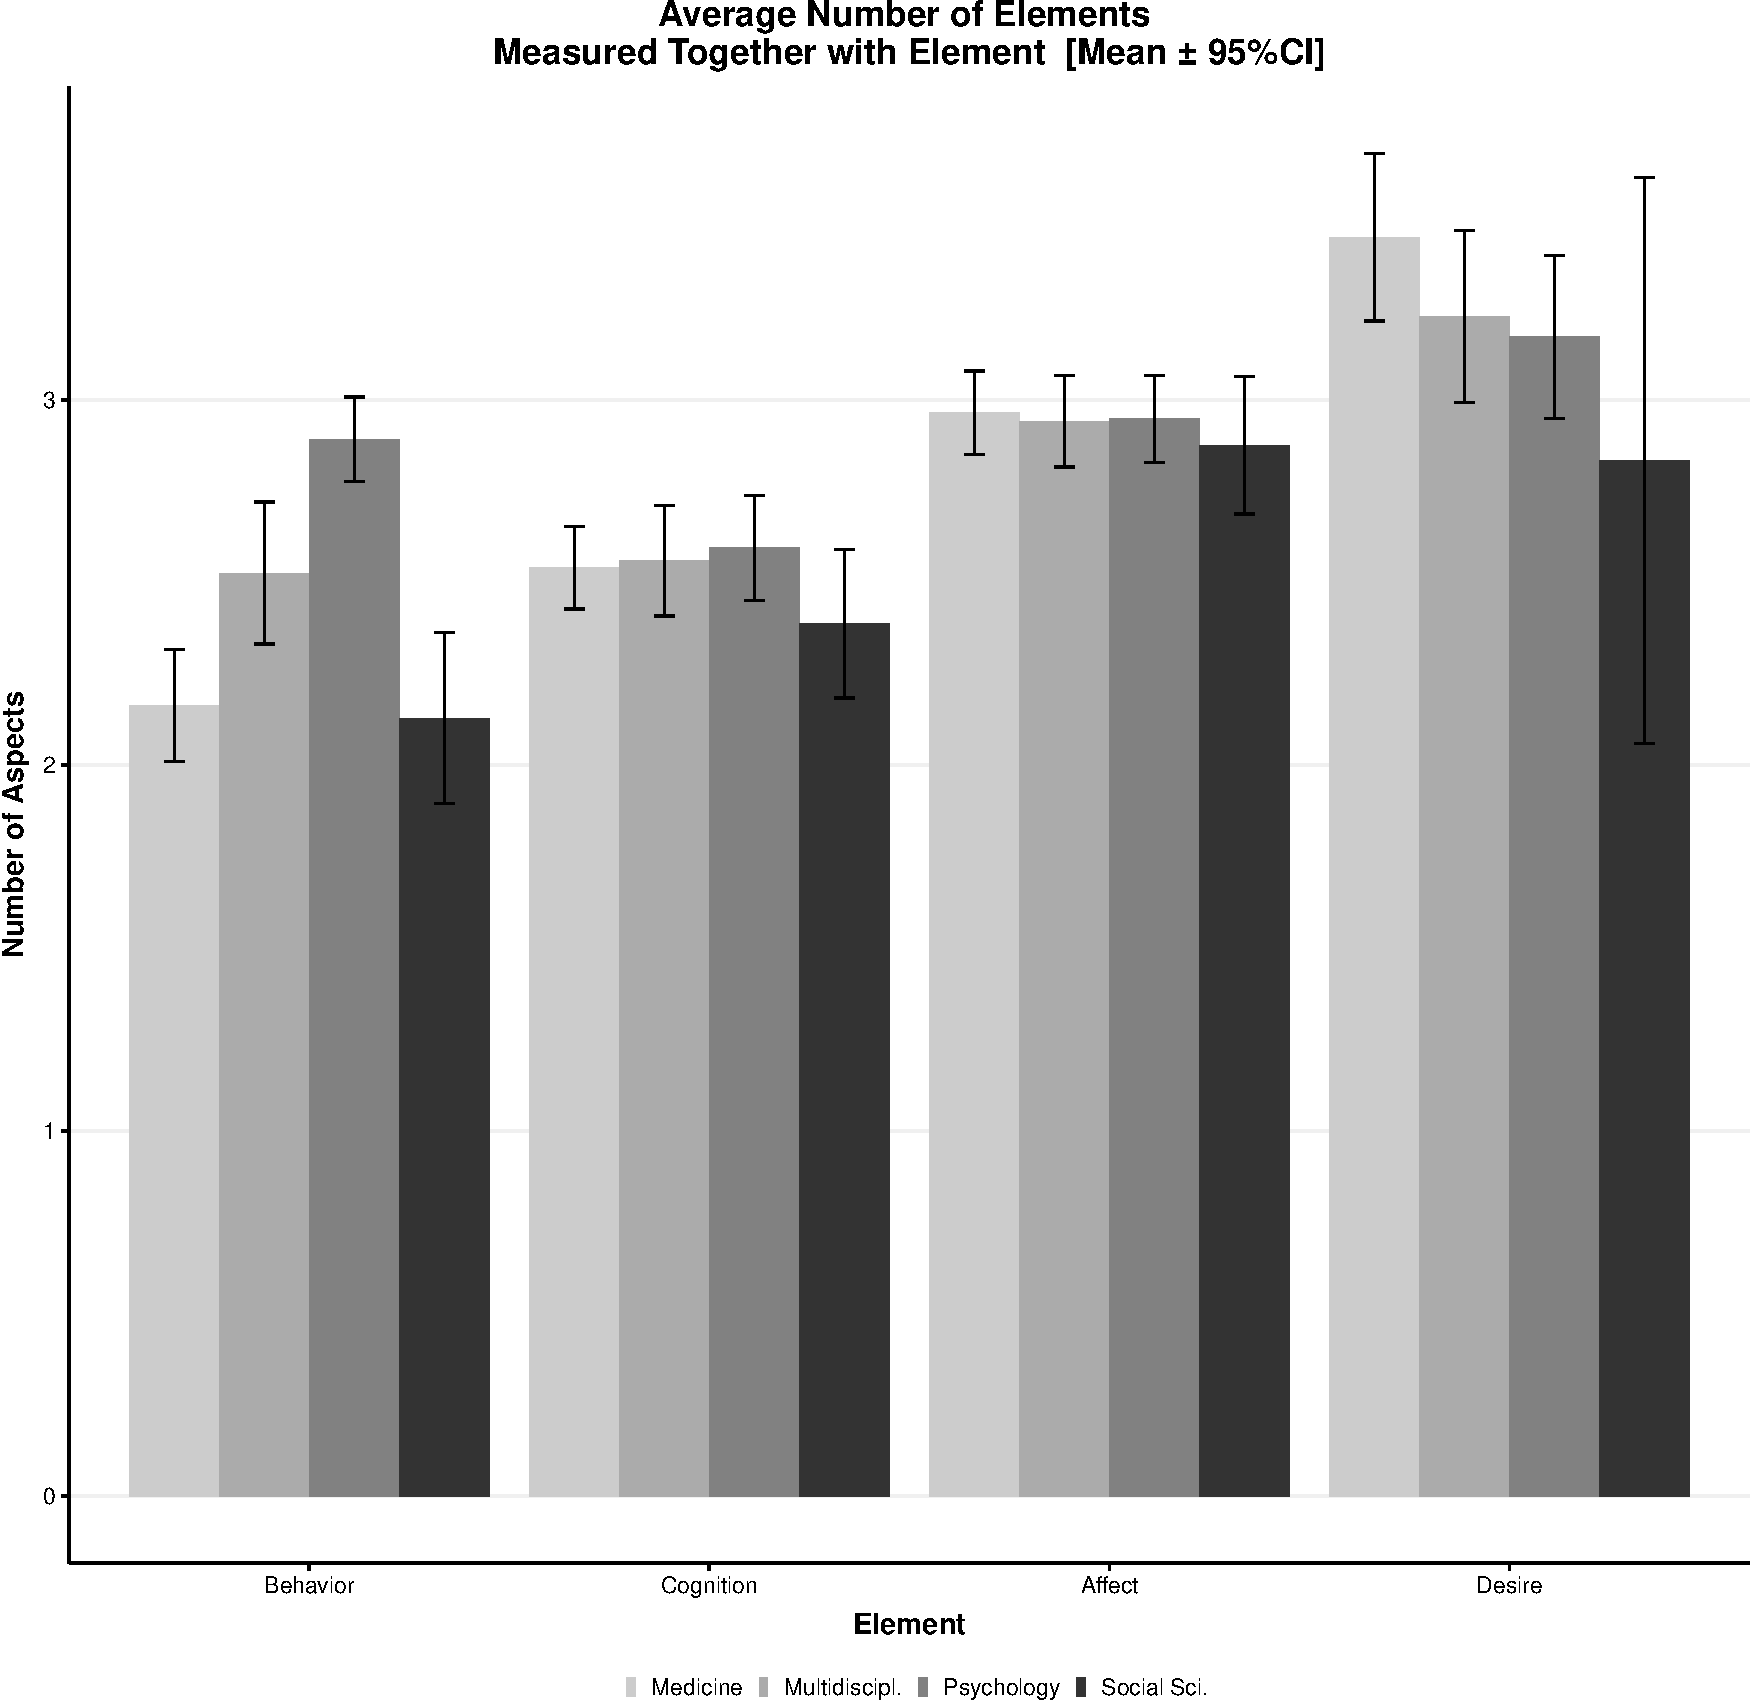
\includegraphics[width=\textwidth]{Figures/FieldElementComp-1}
\caption*{Note that these categories are not mutually exclusive (and thus not independent) because scales can include multiple experience aspects (i.e., higher complexity).}
\label{fig:FieldElementComp}
\end{figure}


\section{Discussion}
\todo[inline]{*Summary*}
%Focus group discussion: behavior, cognition, affect, and desire clearly distinguished in the discussion of what is important in the field for a variety of societal players.
%Behavior and cognition have more expectations from host population and are more visible, affect and desire are more personal (i.e., less visible) but more powerful motor of change.

Literature review: complexity of dimensions and domains widely different between scales, studies, and fields. Cognition and behavior main focus across the board. Desire mostly in more complex measures and conceptualisations.

mention that we only compared between fields -- else too messy.

%% Host-Migrant Interconnectedness:
% Focus on migrant perspective because often disadvantaged position but any interdependent aspect should show up in ABCD + framework can also be used for majority perspective (but not focus of this paper)
Before we move on to the systematic review and our test of the conceptual framework, we would like to remark on our focus on the migrant's rather than the majority group member's experiences. 
While this framework explicitly focuses on the migrant's experience as the structuring experience, this is not meant to put the sole responsibility of ``migration success'' on the newcomer or ignore the interconnectedness of intercultural exchange. We focus on the migrant experience as the structuring element because migrants usually find themselves in disadvantaged positions. 

We would also like to address the issue of interactive acculturation. \citet{Bourhis1997a} and others, have often highlighted that cultural adaptation is essentially interactive and one should not consider the acculturation process of one individual or group without the consideration of the other group and the interaction partners. We agree, and while we address some of these issues explicitly in the framework, we would also like to highlight that within the experience framework aspects of cultural adaptation that are interconnected, co-dependent, or depend on the host majority members likely influence the individual's migration experience. As an example, if a migrant is frequently confronted with exclusion and hostility, this will likely affect their motivations, emotions, thoughts, and behaviors. 
We would also like to highlight that the framework is equally applicable to the cultural adaptation experience of host majority members in their interactions with or perceptions of migrants. Although not the focus of this paper, the same assessments of measures, definitions, and understandings should be able to be conducted with the experience of the majority group.
Additionally, this framework is not meant as an exhaustive or exclusive list of all adaptation aspects but rather offers a structural framework to analyze and understand the broad experience of cultural adaptation.
%Migration is a complex trans-formative experience within different areas of personal- and social life. 


\vspace{1em}
\todo[inline]{*Use of the framework*}
\textbf{Practitioners}: Focus group discussion: good grass-root level validation of the framework.

Useful for considering the concept in its personal complexity and to guide decisions in interventions, as well as monitoring and evaluations. 

\textbf{Researchers}: Literature review: framework good tool to describe measures, empirical work, and fields.

% Novel predictions: Thinking about ABCD aspects allows for new questions about focus, connections, and differences. Why is A, B, C, or D more important? What is the relationship between A, B, C, and D? Are internal aspects (D) more important than external aspects (B)?
\vspace{1em}
\todo[inline]{summary too abstract.}
Moreover, the structural framework also allows for novel questions and predictions. The structure, for example, allows for considerations of the relative importance, the interconnections, or the accessibility of these elements. There might, for example, be theoretical reasons why a certain aspect is more important to a specific issue (e.g., the role of emotions and cognitions to mental health; reference to theory here?). One could also offer process considerations, making theoretical arguments why a certain aspect might precede another or how one aspect might feed back into another (e.g., motivations guiding cognition and affect, which in turn drive behavior; reference to theory here? e.g., theory of reasoned goal pursuit). Another example, for a novel prediction could be a consideration of the accessibility of the individual aspects, where more public aspects, such as behaviors, might be seen as more important to the majority society, whereas more internal aspects such as motivations and goals might be more important to the newcomer (or their group; reference to theory here?). [\Warning\ maybe move to discussion?]

However, there might also be structural patterns one could assess and novel questions one can ask. One might, for example, assess which emotions were most frequently included in measures and definitions of acculturation \citep[e.g., specific emotions such as anger or pride, but also types of emotions, such as positive or negative, or about yourself or others;][]{DeLeersnyder2017}. One might also be interested in co-occurences of contents (e.g., within aspect: identifications and attitudes, but also between aspects: the need for belongingness and emotion of loneliness). It would also allow for conscious considerations of relationships within or between experience aspects. And these types of questions can be asked about past definitions and measurements (i.e., are there patterns in the literature), for a specific field (e.g., which emotions are relevant in the clinical context) or a specific cultural context (e.g., are there specific needs of Syrian refugees in Europe). 

Also offers framework for reflection on study conception and conscious decision of focus on dimensions and domains.

Framework and literature review can also be used as a database to selectively search measures and empirical results.
\subsection{Limitations}
As a psychological model it does not capture physical, cultural, or societal changes as part of the structural. Also ignores measures of integration that outside the agency of the migrant such as length of residence, immigration status, or discrimination experiences.

\subsection{Conclusion}
A person-centered framework based on core facets of the migrants’ experience and the environmental contexts of life domains offers a useful tool for both researchers and practitioners. Qualitative analysis shows embeddedness of conceptualization and systematic review shows utility to structure, and understand the concept of cultural adaptation.

\section{Notes to self}
\begin{itemize}
  \item how much background / literature review?
  \item where does the framework go?
  \item Dimensions and Domains?
  \item new predictions from the framework?
  \item subsubsection order in review?
  \item cluster domains (?)
  \item drop non-empirical work (footnote or SI with comparison to empirical work)
  \item also output percentages for comparison
  \item headers in introduction
  \item life domains (in part) based on Humanitas
\end{itemize}

\printbibliography

\appendix

\section{Search Strategy}
\label{app:AppendixSearchStrategy}

In our search we used an adapted version of the `SPIDER' research tool \citep[e.g.,][]{Cooke2012}. We utilized the \textit{Evaluation} element mainly to exclude articles that were not relevant to the search. The exact search terms used are listed in Table \ref{tab:SearchStrategiesTab}.

\todo[inline]{Re-check search terms.}

\begin{table}
\caption{Search Strategy Cultural Adaptation Review}
\label{tab:SearchStrategiesTab} 
\begin{tabular}{ll}
\hline
Element & Search Terms \\ 
\hline \\ [-0.5em]

% Sample
Sample & 
    (Immigration OR migration OR migrant OR immigration OR refugee) \\ 
    \\ [-0.25em]
    
% Phenomenon of Interest
\begin{tabular}[t]{@{}l@{}}Phenomenon \\of Interest\end{tabular} & 
    \begin{tabular}[t]{@{}l@{}}(acculturation OR enculturation OR transculturation OR \\
    assimilation OR "social integration" OR "cultural adaptation" OR \\
    "cultural adjustment" OR "cultural transition")\end{tabular}  \\ 
    \\ [-0.25em]
    
% Design
Design & 
    \begin{tabular}[t]{@{}l@{}}("measurement tool" OR scale OR instrument OR \\
    questionnaire OR survey OR definition OR inventory)\end{tabular}  \\ 
    \\ [-0.25em]
    
% Evaluation
Evaluation & 
    \begin{tabular}[t]{@{}l@{}}NOT (parent* OR college OR resilience OR treatment OR \\
    intervention OR therapy)\end{tabular}  \\ 
    \\ [-0.25em]
    
% Research Type
Research type * & 
    (quantitative OR qualitative OR "mixed method") \\ [0.75em] 
    \hline

% Note
\multicolumn{2}{l}{* This element was ultimately dropped because it was too sensitive in PsycInfo.}
\end{tabular}
\end{table}


\section{Appendix Title B (EXAMPLE)}
\label{app:AppendixLableB}

These appendices are only here so that I don't loose the template and forget how to insert and reference them in \LaTeX.

As shown in Figure~\ref{fig:FigureAppendix}, these results are impressive. 

\begin{figure}
    \caption{This is my figure caption.}
    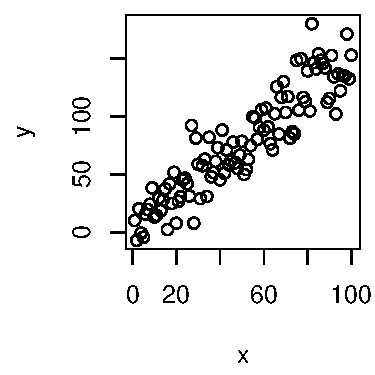
\includegraphics[bb=0in 0in 2.5in 2.5in, height=2.5in, width=2.5in]{Figures/Backup/Figure1.pdf}
    \label{fig:FigureAppendix}
\end{figure}

The detailed results are shown in Table~\ref{tab:DeckedTable}. 

\begin{table}
  \begin{threeparttable}
    \caption{A More Complex Decked Table}
    \label{tab:DeckedTable}
    \begin{tabular}{@{}lrrr@{}}         \toprule
    Distribution type  & \multicolumn{2}{l}{Percentage of} & Total number   \\
                       & \multicolumn{2}{l}{targets with}  & of trials per  \\
                       & \multicolumn{2}{l}{segment in}    & participant    \\ \cmidrule(r){2-3}
                                    &  Onset  &  Coda            &          \\ \midrule
    Categorical -- onset\tabfnm{a}  &    100  &     0            &  196     \\
    Probabilistic                   &     80  &    20\tabfnm{*}  &  200     \\
    Categorical -- coda\tabfnm{b}   &      0  &   100\tabfnm{*}  &  196     \\ \midrule
    \end{tabular}
    \begin{tablenotes}[para,flushleft]
        {\small
            \textit{Note.} All data are approximate.

            \tabfnt{a}Categorical may be onset.
            \tabfnt{b}Categorical may also be coda.

            \tabfnt{*}\textit{p} < .05.
            \tabfnt{**}\textit{p} < .01.
         }
    \end{tablenotes}
  \end{threeparttable}
\end{table}


\end{document}

%% 
%% Copyright (C) 2019 by Daniel A. Weiss <daniel.weiss.led at gmail.com>
%% 
%% This work may be distributed and/or modified under the
%% conditions of the LaTeX Project Public License (LPPL), either
%% version 1.3c of this license or (at your option) any later
%% version.  The latest version of this license is in the file:
%% 
%% http://www.latex-project.org/lppl.txt
%% 
%% Users may freely modify these files without permission, as long as the
%% copyright line and this statement are maintained intact.
%% 
%% This work is not endorsed by, affiliated with, or probably even known
%% by, the American Psychological Association.
%% 
%% This work is "maintained" (as per LPPL maintenance status) by
%% Daniel A. Weiss.
%% 
%% This work consists of the file  apa7.dtx
%% and the derived files           apa7.ins,
%%                                 apa7.cls,
%%                                 apa7.pdf,
%%                                 README,
%%                                 APA7american.txt,
%%                                 APA7british.txt,
%%                                 APA7dutch.txt,
%%                                 APA7english.txt,
%%                                 APA7german.txt,
%%                                 APA7ngerman.txt,
%%                                 APA7greek.txt,
%%                                 APA7czech.txt,
%%                                 APA7turkish.txt,
%%                                 APA7endfloat.cfg,
%%                                 Figure1.pdf,
%%                                 shortsample.tex,
%%                                 longsample.tex, and
%%                                 bibliography.bib.
%% 
%%
%% End of file `./samples/longsample.tex'.
